\chapter{Eksperimen dan Analisis}

\section{Parameter Eksperimen}

Parameter eksperimen ditetapkan untuk mengukur pencapaian tujuan penelitian secara objektif. Pengukuran dikelompokkan ke dalam lima kategori yang mengikuti dua jalur yang dilaporkan, yaitu jalur preprocessing \textit{real-time} dan jalur model TinyML \textit{on-device}, serta satu jalur \textit{pipeline edge-to-cloud} yang dicantumkan sebagai rencana. Target setiap parameter diambil dari rencana pengujian pada Tabel~\ref{tab:pengujian-model} dan Tabel~\ref{tab:pengujian-pipeline}, sedangkan ambangnya bersumber dari standar, jurnal, atau spesifikasi resmi perangkat. Rincian parameter yang diukur adalah sebagai berikut.

\subsubsection{Kualitas Klasifikasi Model}

Parameter ini menilai kemampuan model membedakan detak Normal dan Aritmia pada pasien yang tidak pernah dilihat saat pelatihan. Pembagian \textit{inter-patient} dan pengelompokan kelas AAMI mengikuti de Chazal~\cite{aami_ec57_2012, dechazal_2004} agar hasilnya sebanding dengan literatur. Seluruh metrik dihitung pada DS2 untuk model INT8 yang dijalankan di perangkat, dengan \textit{threshold} hasil kalibrasi data validasi, yaitu \textit{threshold} dengan F1 maksimum. Metrik diturunkan dari \textit{confusion matrix} dengan kelas Aritmia sebagai kelas positif, yaitu \textit{true positive} (TP), \textit{false positive} (FP), \textit{true negative} (TN), dan \textit{false negative} (FN), lalu dirumuskan pada Persamaan~\ref{eq:metrik}~\cite{chicco_2020}.

\begin{align}
\text{Recall} &= \frac{\text{TP}}{\text{TP} + \text{FN}} \nonumber \\
\text{Precision} &= \frac{\text{TP}}{\text{TP} + \text{FP}} \nonumber \\
\text{Specificity} &= \frac{\text{TN}}{\text{TN} + \text{FP}} \nonumber \\
\text{F1} &= \frac{2 \cdot \text{Precision} \cdot \text{Recall}}{\text{Precision} + \text{Recall}} \nonumber \\
\text{MCC} &= \frac{\text{TP} \cdot \text{TN} - \text{FP} \cdot \text{FN}}{\sqrt{(\text{TP} + \text{FP})(\text{TP} + \text{FN})(\text{TN} + \text{FP})(\text{TN} + \text{FN})}}
\label{eq:metrik}
\end{align}

\noindent di mana TP adalah detak aritmia yang diprediksi aritmia, FP adalah detak normal yang diprediksi aritmia, TN adalah detak normal yang diprediksi normal, dan FN adalah detak aritmia yang terlewat. Metrik yang dilaporkan adalah sebagai berikut.
\begin{enumerate}[label=\arabic*)]
  \item \textit{Recall}. Proporsi detak aritmia yang terdeteksi, yaitu kemampuan model untuk tidak melewatkan aritmia.
  \item \textit{Precision}. Proporsi prediksi aritmia yang benar, yaitu kemampuan model untuk tidak memberi alarm palsu pada detak normal.
  \item \textit{Specificity}. Proporsi detak normal yang dikenali sebagai normal.
  \item F1. Rerata harmonik \textit{precision} dan \textit{recall}, yang juga menjadi kriteria kalibrasi \textit{threshold}.
  \item MCC. \textit{Matthews correlation coefficient}, yaitu korelasi antara prediksi dan label yang memakai keempat sel \textit{confusion matrix}, sehingga nilainya hanya tinggi bila kedua kelas dikenali dengan baik~\cite{chicco_2020}.
  \item AUC. Luas di bawah kurva ROC, yaitu kurva pasangan \textit{recall} dan $1 - \textit{specificity}$ untuk seluruh \textit{threshold}, sehingga kemampuan model memisahkan kedua kelas dapat dinilai tanpa bergantung pada satu \textit{threshold}~\cite{chicco_2020}. Nilai AUC juga tidak berubah oleh proporsi kelas, jadi tetap sahih walaupun detak Aritmia hanya sekitar 11\% DS2~\cite{richardson_2024}.
  \item \textit{Accuracy}. Proporsi seluruh prediksi yang benar. Metrik ini tetap dihitung tetapi tidak dijadikan acuan~\cite{chicco_2020}, karena 89,0\% detak DS2 berlabel Normal dan menebak Normal untuk seluruh detak sudah menghasilkan \textit{accuracy} sekitar 0,89.
  \item \textit{Recall} per kelas AAMI dan per pasien. \textit{Recall} kelas S, V, dan F serta median dan rerata \textit{recall} per rekaman, untuk melihat kelas dan pasien yang paling sering terlewat.
  \item Perbandingan dengan model \textit{float32}. F1 model INT8 dibandingkan dengan F1 model \textit{float32} pada DS2 yang identik untuk memastikan kuantisasi tidak menurunkan kualitas. Targetnya mengikuti MLPerf Inference, yaitu kualitas model teroptimasi berada dalam 1\% dari model \textit{float32}~\cite{reddi_2020}, sehingga F1 INT8 minimal 99\% F1 \textit{float32}. F1 dipakai karena \textit{threshold} dikalibrasi dari F1 maksimum.
\end{enumerate}

Metrik kategori ini dilaporkan tanpa ambang lulus karena rencana pengujian tidak menetapkan ambang angka, kecuali perbandingan dengan model \textit{float32}. Kualitas klasifikasi dibandingkan dengan penelitian terkait yang memakai protokol \textit{inter-patient} pada analisis hasil.
% sumber: model/data/processed/test.npz (49.656 detak, y.mean() = 0,1098, Normal 89,02%); model/CLAUDE.md decision "Metrik yang dipantau" (accuracy tidak dipakai)
% sumber: Chicco dan Jurman 2020 (MCC memakai keempat sel, disarankan atas F1 dan accuracy bila threshold tersedia); Richardson dkk. 2024 Summary ("the ROC curve is robust to class imbalance, while the PR curve is highly sensitive to class imbalance"), PR-AUC karena itu tidak dilaporkan di buku (nilainya ada di model/docs/evaluate-walkthrough.md bagian 3b)
% sumber: Reddi dkk. 2020 hlm. 5 ("within 1% of the FP32 reference model's accuracy"); keputusan user 1 Nov 2026: kategori Dampak Kuantisasi digabung ke Kualitas Klasifikasi, hasil DS2 dilaporkan untuk model INT8

\subsubsection{Kinerja di Perangkat}

Parameter ini menilai apakah model INT8 dapat berjalan di ESP32-S3 dalam batas waktu dan memori perangkat.
\begin{enumerate}[label=\arabic*)]
  \item Latensi inferensi per detak. Waktu satu inferensi model INT8 di ESP32-S3. Inferensi harus selesai sebelum detak berikutnya agar \textit{real-time}, sehingga targetnya lebih kecil dari interval antardetak~\cite{tran_2025}.
  \item Pemakaian memori. \textit{Tensor arena}, \textit{heap} bebas, serta pemakaian RAM dan \textit{flash} hasil \textit{build}. \textit{Tensor arena} diukur dengan API TensorFlow Lite Micro~\cite{david_2021}, dan targetnya muat di SRAM perangkat.
  \item Ukuran model INT8. Standar batas ukuran model TinyML belum ditemukan, karena itu ukuran model dinilai terhadap kapasitas memori ESP32-S3~\cite{espressif_esp32s3_wroom1, espressif_esp32s3_datasheet} dengan target muat di \textit{flash} perangkat.
\end{enumerate}
% sumber: Tran dkk. 2025 hlm. 541 (inferensi dibandingkan interval antardetak minimum 400 ms); David dkk. 2021 bagian 5.3 (alokasi arena persisten dan nonpersisten); firmware/platformio.ini (ESP32-S3 N16R8, 16MB flash, 8MB PSRAM)

\subsubsection{Preprocessing di Mikrokontroler}

Parameter ini menilai apakah rantai preprocessing berjalan secara \textit{real-time} pada laju cuplik 360 Hz.
\begin{enumerate}[label=\arabic*)]
  \item Beban komputasi per sampel dan puncak beban. Waktu pemrosesan setiap sampel yang dicatat dengan penghitung mikrodetik perangkat. Pemrosesan per sampel harus selesai dalam satu periode cuplik~\cite{busia_2025}, sehingga targetnya rata-rata beban lebih kecil dari anggaran waktu per sampel.
  \item Jumlah sampel hilang. Jumlah sampel ADC yang tidak sempat diproses. Targetnya tidak ada sampel yang hilang, karena sampel yang hilang merusak interval R-R yang menjadi masukan cabang ritme.
\end{enumerate}
% sumber: Busia dkk. 2025 hlm. 10 ("0.77 ms for each newly acquired sample"); laporan/buku-pa/bab/bab3.tex Subbab Akuisisi Sinyal ECG (antrean ISR, sampel tidak hilang); keputusan user 1 Nov 2026 (uji kesetaraan kode C vs Python dihapus dari buku tahap 1)

\subsubsection{Akuisisi Sinyal Tubuh}

Parameter ini menilai kelayakan sinyal tubuh dari AD8232 sebagai masukan jalur preprocessing. \textit{Flag lead-off} AD8232 tidak menjamin adanya sinyal, karena itu ayunan ADC absolut dijadikan acuan ada tidaknya biopotensial.
\begin{enumerate}[label=\arabic*)]
  \item Ayunan sinyal ADC. Selisih nilai maksimum dan minimum sinyal dalam \textit{count} dan dalam mV ekuivalen masukan AD8232. Ayunan dilaporkan tanpa ambang lulus.
  \item Dengung 50 Hz dan sampel jenuh. Persentase energi pita 50 Hz terhadap energi pita ECG 0,5--40 Hz~\cite{gajdzik_2026} serta jumlah sampel di batas ADC. Keduanya dilaporkan tanpa ambang lulus karena acuan baku untuk ambangnya tidak ditemukan.
  \item Indeks kualitas sinyal per jendela 10 detik. Setiap jendela harus memenuhi syarat detak per menit 40--180, jeda antar-R-\textit{peak} paling lama 3 detik, dan rasio interval R-R terpanjang terhadap terpendek di bawah 2,2. Jendela dinyatakan lolos bila rerata korelasi setiap kompleks QRS terhadap \textit{template} juga minimal 0,66~\cite{syversen_2024}.
\end{enumerate}
% sumber: Syversen dkk. 2024 bagian SQI1 (40-180 bpm, jeda < 3 s, rasio < 2,2, korelasi template 0,66); Gajdzik dkk. 2026 hlm. 59-60 (PLIratio = P 49-51 Hz / P 0,5-40 Hz, tanpa ambang lulus); ambang gerbang kalibrasi (AMBANG_AYUN 60, kontak 60 s, RR 300-1500 ms, |dRR| <= 200 ms) adalah hasil ukur sendiri dan tidak dijadikan parameter atas keputusan user 1 Nov 2026, diuji sebagai uji fungsi di butir Gerbang Kalibrasi

\subsubsection{\textit{Pipeline Edge-to-Cloud}}

Parameter ini menilai kontinuitas data hasil klasifikasi dari perangkat ke \textit{cloud}. Bufer lokal di sisi \textit{edge} mempertahankan kontinuitas data ketika koneksi putus~\cite{escobedo_2026, tipparaju_2021}, karena detak yang hilang bertepatan dengan kejadian aritmia tidak dapat direkonstruksi di sisi \textit{cloud}. Target kategori ini dicantumkan sebagai rencana, karena hasil pengujian \textit{pipeline} belum termasuk dalam laporan tahap ini.
\begin{enumerate}[label=\arabic*)]
  \item \textit{Packet Delivery Success Rate} (PDSR). Persentase paket yang dikonfirmasi PUBACK pada percobaan pertama, dengan target minimal 95\%.
  \item Latensi \textit{end-to-end}. Waktu dari terjadinya detak hingga data tersedia di \textit{cloud}, dengan target median paling lama 2 detik. Persentil ke-95 (p95) dilaporkan agar ekor sebarannya ikut terlihat.
  \item Jumlah entri \textit{ring buffer}. Isi bufer lokal saat \textit{streaming} normal dan saat koneksi putus, dengan target tidak \textit{overflow} dalam kapasitas $\pm$27.000 rekaman.
  \item Data hilang saat putus koneksi. Jumlah detak yang tidak sampai ke \textit{cloud} setelah koneksi pulih, dengan target tidak ada.
  \item Waktu \textit{flush}. Durasi sejak koneksi pulih hingga bufer terkuras, dengan target paling lama 60 detik.
  \item Paket ganda. Duplikat akibat pengiriman ulang QoS 1, dengan target dikenali dan diabaikan di sisi \textit{cloud}.
\end{enumerate}
% sumber: laporan/buku-pa/bab/bab3.tex tab:pengujian-pipeline

\section{Karakteristik Data}

Karakteristik data diuraikan dalam empat butir. Butir pertama membahas data sekunder untuk pelatihan dan pengujian model, lalu berturut-turut data primer hasil rekaman perangkat, sumber sinyal \textit{replay}, dan penyelarasan pemrosesan antara komputer dan perangkat.

\subsubsection{Data Sekunder untuk Pelatihan dan Pengujian}

Data sekunder utama adalah MIT-BIH \textit{Arrhythmia Database} yang terdiri atas 48 rekaman dengan frekuensi sampel 360 Hz pada sadapan MLII~\cite{moody_mark_2001}. Rekaman 102 dan 104 dikeluarkan karena tidak memiliki kanal MLII, sedangkan rekaman 107 dan 217 dikeluarkan karena berisi detak alat pacu jantung, dan tersisa 44 rekaman. Label anotasi dipetakan ke kelas biner Normal dan Aritmia sesuai Tabel~\ref{tab:pemetaan-label}. Rekaman dibagi menjadi DS1 dan DS2 mengikuti pembagian \textit{inter-patient} de Chazal~\cite{dechazal_2004}, dan lima rekaman DS1, yaitu 101, 114, 201, 220, dan 223, dipisahkan sebagai data validasi (VAL).
% sumber: model/config.py (FS = 360, PACED_EXCLUDED = [102, 104, 107, 217], VAL_RECORDS = [101, 114, 201, 220, 223], DS2 22 rekaman); model/CLAUDE.md Fase 0 (48 record)

Setiap rekaman DS1 ditumpuk menjadi tiga salinan, yaitu satu salinan bersih dan dua salinan yang posisi segmentasinya digeser dengan \textit{jitter} empiris. Besar pergeserannya diambil ulang dari sebaran \textit{error} detektor R-\textit{peak} yang diukur sendiri, mengadaptasi gagasan augmentasi \textit{jitter}~\cite{dias_2021}. DS2 tidak diberi \textit{jitter} dan karena itu mewakili anotasi tanpa \textit{error} segmentasi. DS2 juga dipakai sebagai ukuran pada ablasi yang menentukan ukuran \textit{window} dan jumlah salinan \textit{jitter}, sedangkan pemilihan \textit{epoch} dan \textit{threshold} hanya memakai VAL. Angka DS2 pada bab ini karena itu bukan data uji yang sepenuhnya belum tersentuh untuk dua keputusan pertama. Komposisi seluruh himpunan data ditunjukkan pada Tabel~\ref{tab:dataset}.
% sumber: model/config.py (JITTER_MODEL = "empiris", JITTER_SALINAN = 2); model/CLAUDE.md decision "Augmentasi jitter", "Model jitter", "Database LATIH" (mitdb saja) dan "Validation set"

\begin{table}[!ht]
  \centering
  \caption{Komposisi himpunan data sekunder}
  \label{tab:dataset}
  \setstretch{1.0}
  \setlength{\tabcolsep}{4pt}
  \renewcommand{\arraystretch}{1.15}
  \small
  \begin{tabular}{>{\RaggedRight\arraybackslash}p{1.9cm}>{\RaggedRight\arraybackslash}p{2.9cm}>{\RaggedRight\arraybackslash}p{3.2cm}>{\centering\arraybackslash}p{1.5cm}>{\RaggedRight\arraybackslash}p{3.0cm}}
    \toprule
    \textbf{Himpunan} & \textbf{Sumber} & \textbf{Jumlah Data} & \textbf{Aritmia (\%)} & \textbf{Kegunaan} \\
    \midrule
    DS1 latih & 17 rekaman MIT-BIH & 121.857 baris (40.619 detak $\times$ 3 salinan) & 10,1 & Pelatihan model \\
    VAL & 5 rekaman MIT-BIH (bagian DS1) & 31.047 baris (10.349 detak $\times$ 3 salinan) & 10,1 & Pemilihan \textit{epoch} dan kalibrasi \textit{threshold} \\
    DS2 & 22 rekaman MIT-BIH & 49.656 detak & 11,0 & Pengujian utama \\
    \bottomrule
  \end{tabular}
\end{table}
% sumber: numpy atas model/data/processed/train.npz (152.904 baris, 22 rekaman, 50.968 detak x 3; VAL 31.047 baris = 10.349 x 3; latih 121.857 = 40.619 x 3; aritmia 10,11%), test.npz (49.656, 22 rekaman, 10,98%)

Proporsi aritmia pada DS1 maupun DS2 hanya berada di kisaran 10--11\% (Tabel~\ref{tab:dataset}), dan DS1 secara keseluruhan memuat 22 rekaman dengan 152.904 baris setelah augmentasi. Ketidakseimbangan kelas ini menjadi alasan \textit{class weight} dipakai saat pelatihan dan \textit{accuracy} tidak dijadikan acuan.
% sumber: model/data/processed/train.npz (152.904 baris); model/CLAUDE.md decision "Strategi imbalance" (class_weight balanced)

\subsubsection{Data Primer dari Perangkat}

Data primer berupa rekaman sinyal mentah dari modul AD8232 yang dicuplik ADC ESP32-S3 pada 360 Hz dan disimpan sebagai berkas CSV berisi nilai \textit{count} ADC 12-bit melalui alur perekaman di perangkat. Rekaman yang sempat dijeda terdiri atas beberapa segmen, dan durasinya dihitung dari jumlah sampel seluruh segmen tanpa waktu jeda. Rekaman yang diambil selama pengembangan hanya dipakai untuk menyusun prosedur perekaman dan menguji alat analisis, dan tidak dilaporkan sebagai hasil. Data primer yang dilaporkan berasal dari pengujian rekaman resmi, yaitu satu sesi perekaman tanpa jeda pada 22 Oktober 2026 sekitar pukul 12.38--12.54 WIB. Perangkat menyimpan sesi tersebut sebagai empat rekaman berurutan, yaitu tiga rekaman 300 detik dan satu rekaman 27,1 detik, dengan total 927,1 detik. Rekaman berasal dari satu subjek sehat, yaitu penulis sendiri dengan kode S01, dengan konfigurasi Lead II dan elektroda \textit{wet-gel}. Pengambilan data ini bukan uji klinis.
% sumber: model/data/recordings/20261022-1256-rekam-001.csv dan -002.csv, 20261022-1257-rekam-003.csv dan -004.csv (header n=108000, 108000, 108000, 9771; lanjutan=001..003 celah=0; 9771 / 360 = 27,1 detik; total 333.771 sampel = 927,1 detik); model/data/recordings/README.md Catatan per sesi (22 Okt 2026 siang, MLII, powerbank, elektroda baru); jam: sesi berakhir sebelum status board 12:55:02 WIB sesudah USB dicolok, dikurangi 927 detik (perkiraan, berkas dinamai menurut jam tarik 12:56-12:57); subjek = penulis (keputusan user 22 Okt 2026)
% sumber: rekaman uji coba 10 Sep - 11 Okt 2026 (27 berkas) diarsipkan di model/data/arsip/rekaman-uji-coba/README.md dan tidak dipakai sebagai hasil

Penempatan elektroda mengikuti konfigurasi Lead II sebagaimana ditunjukkan pada Gambar~\ref{fig:4-elektroda}.

% PLACEHOLDER-GAMBAR fig:4-elektroda  (foto user, bukan Claude)
% Jenis      : foto dokumentasi, portrait
% Pesan      : letak tiga elektroda wet-gel untuk Lead II
% Elemen     : torso dari bahu sampai pinggang TANPA wajah, tato, atau penanda identitas; RA di bawah selangka kanan; LA di bawah rusuk kiri; RL di bawah rusuk kanan sebagai referensi
% Alur baca  : atas ke bawah, RA, lalu LA, lalu RL
% Teks       : label persis "RA", "LA", "RL"
% Bahan repo : model/docs/akuisisi-walkthrough.md §1
% Ukuran     : height=0.4\textheight,keepaspectratio
\begin{figure}[!ht]
  \centering
  \PlaceholderGambar{Foto dokumentasi}{posisi elektroda RA, LA, dan RL pada torso subjek tanpa wajah}
  \caption{Posisi elektroda Lead II}
  \label{fig:4-elektroda}
\end{figure}

Pada Gambar~\ref{fig:4-elektroda}, sumbu dari RA ke LA meniru sadapan MLII yang dipakai MIT-BIH, agar morfologi QRS rekaman perangkat sebanding dengan data latih.
% sumber: model/docs/akuisisi-walkthrough.md §1 (RA bawah selangka kanan, LA bawah rusuk kiri, RL bawah rusuk kanan sebagai referensi; sumbu merah ke kuning meniru MLII)

Rekaman yang tidak memenuhi kriteria kualitas sinyal tetap disimpan karena menjadi bukti dalam mendiagnosis gangguan akuisisi. Kualitas setiap rekaman dinilai dari ayunan sinyal ADC absolut, kandungan dengung jala-jala, jumlah R-\textit{peak} terdeteksi, dan indeks kualitas sinyal per jendela 10 detik.
% sumber: model/CLAUDE.md Jebakan "Telemetri akuisisi bisa berbohong"; model/docs/akuisisi-walkthrough.md §6 dan §8

\subsubsection{Sumber Sinyal \textit{Replay}}

Untuk menguji jalur hilir secara deterministik tanpa bergantung pada elektroda, perangkat dilengkapi sumber sinyal \textit{replay} yang dipilih dari menu Sumber sinyal. Sumber yang dipakai pada seluruh pengujian bab ini adalah 2.400 sampel pertama sinyal mentah rekaman 208 dari DS1 atau sekitar 6,67 detik, yang dikonversi sekali menjadi nilai \textit{count} ADC saat \textit{setup}. Ketika \textit{replay} aktif, \textit{timer interrupt} menyalin nilai dari tabel tersebut sebagai pengganti pembacaan ADC, sedangkan filter, deteksi R-\textit{peak}, segmentasi, inferensi, dan pengiriman MQTT tidak berubah sama sekali. Karena hanya sumber sampel yang diganti, hasil pengukuran pada jalur hilir dapat dijadikan acuan untuk sinyal yang berasal dari ADC. Catatannya, syarat lama kontak, syarat R-R, dan status \textit{lead-off} pada gerbang kalibrasi dilewati selama \textit{replay}, dan laju detaknya sekitar 1,6 detak per detik. Sumber \textit{replay} rekaman tersimpan juga tersedia, tetapi tidak dipakai pada pengujian yang dilaporkan.
% sumber: firmware/test/golden_ref.h (record 208 DS1, GOLDEN_N 2400, golden_raw); 2400 / 360 = 6,67 detik; firmware/src/akuisisi.cpp on_timer() dan sim_counts (tabel replay acuan); model/docs/firmware-walkthrough.md §5c "Terukur di board" (11 beat per putaran 6,67 detik, 1,58 beat/detik)

Satu putaran sinyal \textit{replay} memuat 9 detak beranotasi, tetapi perangkat mengeluarkan 11 detak per putaran karena sambungan antarputaran menghasilkan dua detak tambahan. Rekaman 208 juga bersifat aritmik dan karena itu tidak dapat melewati gerbang R-R pada fase kalibrasi. Pada \textit{firmware} akhir, pelewatan gerbang tersebut melekat pada sumber \textit{replay} dan berhenti begitu sumber kembali ke sensor, jadi tidak dapat terbawa ke perekaman sinyal tubuh.
% sumber: firmware/test/golden_ref.h (GOLDEN_N_BEAT 9); model/docs/firmware-walkthrough.md §5c "Terukur di board" (11 beat per putaran, akuntansi MQTT pakai 11); model/docs/mqtt-walkthrough.md §3.1b (replay record 208 aritmik, gerbang kalibrasi dilewati selama replay); firmware/src/gerbang.cpp gerbang_nilai_fase() (bypass replay)

\subsubsection{Penyelarasan Pemrosesan antara Komputer dan Perangkat}

Model hanya berlaku di perangkat apabila \textit{window} yang diterimanya identik dengan \textit{window} saat pelatihan. Filter Butterworth pada kedua sisi bersifat kausal dengan koefisien SOS yang sama, karena koefisien untuk kode C dihasilkan otomatis dari Python ke berkas \textit{header} C. Filter kausal menimbulkan \textit{group delay} sebesar 4 sampel, dan pergeseran ini tidak dikoreksi melainkan dipelajari model. Puncak R karena itu berada di indeks 132 pada \textit{window} 256 sampel, yaitu 128 sampel sebelum R ditambah 4. Setiap \textit{window} dinormalisasi \textit{z-score} secara mandiri, dan model INT8 beserta \textit{threshold} 0,80 dibawa ke \textit{firmware} melalui berkas \textit{header} C yang juga dihasilkan otomatis.
% sumber: firmware/include/ecg_preproc.h (GENERATED oleh model/scripts/export_golden.py, ECG_WIN_PRE 128, ECG_WIN_POST 128, ECG_GROUP_DELAY 4); model/config.py (R_IN_WINDOW = WIN_PRE + 4); firmware/include/model_int8.h (GENERATED oleh export_model_h.py, ECG_THRESHOLD 0.8f); model/CLAUDE.md Jebakan "Group delay filter kausal"

Di perangkat, posisi R-\textit{peak} berasal dari detektor Pan-Tompkins, bukan dari anotasi. Keluaran detektor karena itu dikompensasi sebesar 38 sampel, dicari puncak sebenarnya dalam rentang $\pm$25 sampel, lalu dikurangi \textit{group delay} 4 sampel, agar puncak R mendarat di indeks yang sama dengan data latih.

% sumber: firmware/include/ecg_preproc.h (ECG_PT_OFFSET 38, ECG_PT_REFINE 25, ECG_GROUP_DELAY 4); model/CLAUDE.md decision "Segmentasi on-device"; firmware/test/golden_ref.h

\section{Tempat Ujicoba}

Seluruh uji dilakukan di lingkungan non-klinis. Perekaman sinyal tubuh dilakukan di Laboratorium MSECT, Politeknik Elektronika Negeri Surabaya, dengan subjek duduk diam dan perangkat dicatu \textit{powerbank}, jadi tidak ada sambungan listrik ke jala-jala selama perekaman.
% sumber: model/docs/akuisisi-walkthrough.md §1 dan §3 (powerbank, USB laptop dicabut, subjek duduk diam)
% sumber: tempat perekaman resmi 22 Okt 2026 = Lab MSECT PENS (keterangan user 22 Okt 2026)

Pelatihan model, ablasi, kuantisasi, dan uji unit kode C yang tidak memerlukan perangkat keras dijalankan di komputer pribadi. Pemisahan ini dimungkinkan karena tahap tersebut hanya membutuhkan data sekunder dan daya komputasi, sedangkan uji yang melibatkan sinyal tubuh memerlukan perangkat keras.


\section{Waktu Ujicoba}

Kegiatan eksperimen berlangsung sejak Agustus 2026. Rentang setiap kegiatan pada Tabel~\ref{tab:waktu-ujicoba} disusun dari catatan pengembangan, yaitu riwayat \textit{commit} repositori dan nama berkas rekaman, dan dapat berbeda beberapa hari dari tanggal percobaan yang sebenarnya.

\begin{table}[!ht]
  \centering
  \caption{Waktu pelaksanaan kegiatan eksperimen}
  \label{tab:waktu-ujicoba}
  \setstretch{1.0}
  \setlength{\tabcolsep}{4pt}
  \renewcommand{\arraystretch}{1.15}
  \small
  \begin{tabularx}{\linewidth}{>{\RaggedRight\arraybackslash}X>{\RaggedRight\arraybackslash}p{4.4cm}}
    \toprule
    \textbf{Kegiatan} & \textbf{Rentang Waktu} \\
    \midrule
    Pengembangan model, yaitu penyiapan data, pelatihan, evaluasi, kuantisasi, dan ekspor & 24 Agustus -- 10 September 2026 \\
    % sumber: git log 3747551 (2026-08-24, scaffolding pipeline training) sampai ea78eb7 (2026-09-10, Fase 8)
    \textit{Port} preprocessing ke kode C, inferensi di perangkat, alur hidup, dan \textit{firmware} utama & 10 -- 12 September 2026 \\
    % sumber: git log 8eaf44e (2026-09-10, golden reference) sampai 7698c58 (2026-09-12, firmware produksi)
    Perekaman uji coba sinyal tubuh untuk menyusun prosedur akuisisi, pada \textit{breadboard} dan rangkaian berpeta pin PCB & 10 September -- 11 Oktober 2026 \\
    % sumber: model/data/arsip/rekaman-uji-coba/README.md (27 rekaman uji coba 20260910-1938.csv sampai 20261011-1834.csv, bukan hasil)
    Biaya segmentasi di perangkat, ketahanan terhadap \textit{jitter}, dan penguncian \textit{window} & 12 -- 18 September 2026 \\
    % sumber: git log fce7cd1 (2026-09-12, Fase 6b) sampai cf5f5d5 (2026-09-18, retrain window 256)
    Sumber sinyal \textit{replay} & 16 -- 18 September 2026 \\
    % sumber: git log 50dc8d2 (2026-09-16, desain pengukuran daya) sampai 47ca6e6 (2026-09-18, replay golden_raw)
    Ablasi fitur dan regime pelatihan & 19 September 2026 \\
    % sumber: git log 03c77f2 sampai 2acc531 (seluruhnya 2026-09-19)
    Pengukuran ulang segmentasi di perangkat dengan model akhir & 13 Oktober 2026 \\
    % sumber: model/docs/segmentasi-deteksi-walkthrough.md §3 ("kondisi ukur: skrip yang sama, 13 Okt 2026")
    \textit{Firmware} modular dengan antarmuka perangkat, uji perangkat dan uji integrasi di \textit{board} & 13 Oktober 2026 \\
    % sumber: git log 1fa4235 (2026-10-13, satu main.cpp pin map PCB, test perangkat), 9ba6498 (2026-10-13, main.cpp dipecah per modul), b012fa6 (2026-10-13, tangga ukur daya mandiri), 7476063 dan bca5773 (2026-10-13, menu), f6042b5 (2026-10-13, REC/JEDA di layar, rekam dengan jeda, board 29/29 dan native 23/23)
    Pengukuran waktu stabil sinyal tubuh dan pengujian gerbang kalibrasi dengan sinyal tubuh & 21 -- 22 Oktober 2026 \\
    % sumber: model/data/recordings/README.md Catatan per sesi (21 Okt dan dua sesi 22 Okt); model/artifacts/metrics/kualitas/*.csv; model/docs/mqtt-walkthrough.md §3.1c (uji gerbang kontak 22 Okt 2026)
    Pengujian rekaman sinyal tubuh resmi & 22 Oktober 2026 \\
    % sumber: model/data/recordings/20261022-1256-rekam-001.csv sampai 20261022-1257-rekam-004.csv (ditarik 22 Okt 2026)
    \bottomrule
  \end{tabularx}
  \par\vspace{2pt}{\footnotesize\raggedright Keterangan: antarmuka perangkat mencakup layar, menu, dan perekaman berjeda. Kegiatan 13 Oktober 2026 memakai rangkaian uji dengan peta pin PCB.\par}
\end{table}

Pengembangan model mendahului pekerjaan perangkat keras (Tabel~\ref{tab:waktu-ujicoba}), dan sebagian kegiatan berjalan beririsan karena hasil satu jalur langsung dipakai jalur lain. Hasil yang dilaporkan pada bab ini dikumpulkan sampai 13 Oktober 2026, kecuali pengukuran waktu stabil, pengujian gerbang kalibrasi, dan pengujian rekaman sinyal tubuh resmi pada 21--22 Oktober 2026. Segmentasi di perangkat diukur ulang dengan model akhir pada 13 Oktober 2026.
% sumber: model/data/recordings/README.md (rekaman resmi dimulai 13 Okt 2026); model/docs/segmentasi-deteksi-walkthrough.md §3 (13 Okt 2026)


\section{Spesifikasi Peralatan Ujicoba}

Peralatan yang digunakan terdiri atas perangkat keras dan perangkat lunak. Spesifikasi perangkat keras beserta kegunaannya ditunjukkan pada Tabel~\ref{tab:perangkat-keras-uji}.

\begin{table}[!ht]
  \centering
  \caption{Spesifikasi perangkat keras ujicoba}
  \label{tab:perangkat-keras-uji}
  \setstretch{1.0}
  \setlength{\tabcolsep}{4pt}
  \renewcommand{\arraystretch}{1.15}
  \small
  \begin{tabularx}{\linewidth}{>{\RaggedRight\arraybackslash}p{2.4cm}>{\RaggedRight\arraybackslash}X>{\RaggedRight\arraybackslash}X}
    \toprule
    \textbf{Komponen} & \textbf{Spesifikasi} & \textbf{Kegunaan} \\
    \midrule
    Mikrokontroler & \textit{Board} kompatibel ESP32-S3-DevKitC-1, modul ESP32-S3-WROOM-1-N16R8 (\textit{flash} 16 MB, PSRAM 8 MB) & Akuisisi, preprocessing, dan inferensi \\
    % sumber: firmware/platformio.ini (board, komentar 16MB flash 8MB PSRAM)
    Sensor & Modul AD8232, single-lead Lead II, elektroda \textit{wet-gel} & Akuisisi sinyal tubuh \\
    Perakitan & Rangkaian uji berpeta pin PCB (Tabel~\ref{tab:pin-map}) dengan AD8232, TFT ST7789, \textit{buzzer} A18009, tiga tombol, dan LED \textit{NeoPixel} & Uji perangkat, uji integrasi, dan perekaman sinyal tubuh \\
    % sumber: firmware/include/perangkat.h (pin map PCB, ADC1_CHANNEL_0 = GPIO 1); firmware/README.md (board di atas PCB rev1, pin map); riwayat pin rangkaian uji coba di model/data/arsip/rekaman-uji-coba/README.md
    Perakitan awal & \textit{Breadboard}, keluaran AD8232 ke GPIO 8, LO+/LO$-$ ke GPIO 17/7 & Uji model di perangkat, September 2026 \\
    % sumber: riwayat pin breadboard (KANAL_EKG ADC1_CHANNEL_7 = GPIO 8, LO+ 17, LO- 7) di versi lama firmware/src/main.cpp sebelum git 1fa4235; uji test_inference 18 Sep dan uji pipeline 19 Sep 2026 memakai sinyal replay sehingga tidak bergantung pin ADC
    Catu daya & \textit{Powerbank}; USB komputer & Perekaman sinyal tubuh; uji perangkat \\
    % sumber: model/docs/akuisisi-walkthrough.md §1 (daya powerbank) dan §7 (dengung besar bila USB laptop tertancap)
    Komputer & Intel Core i5-12450H (12 \textit{thread}), memori 15 GiB, Debian GNU/Linux 13 & Pelatihan model, ablasi, dan uji unit kode C \\
    % sumber: lscpu (Model name 12th Gen Intel(R) Core(TM) i5-12450H, CPU(s) 12); free -h (Mem total 15Gi); /etc/os-release (Debian GNU/Linux 13 (trixie))
    \bottomrule
  \end{tabularx}
  \par\vspace{2pt}{\footnotesize\raggedright Keterangan: dua catu daya pada baris Catu daya berpasangan urut dengan dua kegunaannya.\par}
\end{table}

Dua rakitan dipakai bergantian pada Tabel~\ref{tab:perangkat-keras-uji}. Uji model di perangkat pada September 2026 memakai rakitan \textit{breadboard} awal, sedangkan uji perangkat dan uji integrasi pada Oktober 2026 memakai rangkaian dengan peta pin PCB. Perbedaan rakitan ini tidak memengaruhi hasil uji model, karena uji tersebut memakai sinyal \textit{replay} yang menggantikan pembacaan ADC. Catu daya juga berganti menurut pengujiannya. \textit{Powerbank} dipakai saat perekaman agar dengung jala-jala 50 Hz dari catu USB komputer tidak masuk, sedangkan USB komputer dipakai pada uji yang membaca serial.

Rakitan perangkat dengan peta pin PCB yang dipakai pada uji perangkat dan perekaman sinyal tubuh ditunjukkan pada Gambar~\ref{fig:4-foto-rakitan}.

% PLACEHOLDER-GAMBAR fig:4-foto-rakitan  (foto user, bukan Claude)
% Jenis      : foto perangkat, landscape
% Pesan      : susunan fisik rakitan perangkat yang dipakai uji perangkat dan perekaman
% Elemen     : papan ESP32-S3 N16R8; modul AD8232 dengan kabel elektroda RA LA RL; layar TFT ST7789 menyala menampilkan layar pemantauan;
%              modul buzzer pasif A18009; tombol B1 B2 B3; catu powerbank
% Alur baca  : kiri ke kanan, dari catu daya, ESP32-S3 dengan layar dan tombol, lalu AD8232 dan kabel elektroda
% Teks       : label opsional pada foto persis "ESP32-S3", "AD8232", "TFT", "Buzzer", "B1", "B2", "B3", "RA", "LA", "RL"
% Bahan repo : firmware/include/perangkat.h (pin map); firmware/README.md bagian Pin map; model/docs/akuisisi-walkthrough.md §1
% Ukuran     : width=\linewidth,keepaspectratio. Tanpa orang, wajah, atau identitas
% KONFIRMASI PENULIS: rakitan fisik ini PCB rev1 atau breadboard dengan peta pin PCB; sesuaikan caption bila perlu
\begin{figure}[!ht]
  \centering
  \PlaceholderGambar{Foto perangkat}{rakitan ESP32-S3 dengan AD8232, TFT, \textit{buzzer}, tombol, dan kabel elektroda}
  \caption{Rakitan perangkat pada ujicoba}
  \label{fig:4-foto-rakitan}
\end{figure}

Pada Gambar~\ref{fig:4-foto-rakitan}, keluaran AD8232 dihubungkan ke ESP32-S3 bersama layar TFT, modul \textit{buzzer}, dan tombol B1 sampai B3, sedangkan kabel elektroda RA, LA, dan RL keluar dari modul AD8232 menuju subjek.

Versi perangkat lunak yang digunakan ditunjukkan pada Tabel~\ref{tab:perangkat-lunak-uji}.

\begin{table}[!ht]
  \centering
  \caption{Versi perangkat lunak ujicoba}
  \label{tab:perangkat-lunak-uji}
  \setstretch{1.0}
  \setlength{\tabcolsep}{4pt}
  \renewcommand{\arraystretch}{1.15}
  \small
  \begin{tabular}{>{\RaggedRight\arraybackslash}p{4.4cm}>{\RaggedRight\arraybackslash}p{3.4cm}>{\RaggedRight\arraybackslash}p{4.8cm}}
    \toprule
    \textbf{Perangkat Lunak} & \textbf{Versi} & \textbf{Kegunaan} \\
    \midrule
    Python & 3.11.9 & Pengembangan model \\
    TensorFlow & 2.21.0 & Pelatihan dan kuantisasi INT8 \\
    NumPy & 2.4.6 & Komputasi metrik \\
    SciPy & 1.17.1 & Filter Butterworth \\
    wfdb & 4.3.1 & Membaca basis data PhysioNet \\
    % sumber: model/.venv/bin/python -c "import tensorflow,numpy,scipy,wfdb; print(...)" -> 2.21.0 2.4.6 1.17.1 4.3.1; model/.python-version 3.11.9
    pyserial & 3.5 & Membaca rekaman lewat serial \\
    % sumber: model/.venv/bin/python -c "import serial; print(serial.__version__)" -> 3.5; model/requirements.txt (pyserial); dashboard/ukur_pipeline.py dan model/scripts/pull_recording.py
    PlatformIO Core & 6.2.0 & \textit{Build}, \textit{flash}, dan uji \textit{firmware} \\
    % sumber: pio --version
    Platform espressif32 & 7.0.1 & Platform ESP32-S3 \\
    Arduino-ESP32 & 2.0.17 (paket 3.20017.241212) & \textit{Framework firmware} \\
    % sumber: pio pkg list -e esp32-s3 (espressif32 @ 7.0.1, framework-arduinoespressif32 @ 3.20017.241212); ~/.platformio/packages/framework-arduinoespressif32/cores/esp32/core_version.h (ARDUINO_ESP32_GIT_DESC 2.0.17)
    Chirale\_TensorFLowLite & 2.0.0 & Inferensi TensorFlow Lite Micro \\
    % sumber: pio pkg list -e esp32-s3 (Chirale_TensorFLowLite @ 2.0.0)
    \bottomrule
  \end{tabular}
\end{table}

Tabel~\ref{tab:perangkat-lunak-uji} mencantumkan versi setiap perangkat lunak secara persis karena berkas kebutuhan Python pada repositori tidak mematok versi \textit{library}. Dengan versi tersebut, eksperimen dapat diulang pada lingkungan yang sama.
% sumber: model/requirements.txt (numpy, scipy, wfdb, tensorflow tanpa nomor versi)

\subsection{Validitas Pengukuran}

Beberapa alat ukur pada eksperimen ini terbukti dapat memberi angka yang salah tanpa pesan kesalahan apa pun. Tiga sumber \textit{error} pengukuran yang ditemukan selama pengembangan beserta penanganannya diuraikan pada butir berikut, agar angka pada hasil eksperimen dapat dinilai keabsahannya.
\begin{enumerate}
  \item Membuka \textit{port} serial me-\textit{reset} perangkat. \textit{Library} pyserial menegaskan sinyal DTR dan RTS saat \textit{port} dibuka, ESP32-S3 pun \textit{reset}, dan pengaturan yang sudah dikirim seperti \textit{replay} ikut hilang. Penanganannya adalah menonaktifkan DTR dan RTS sebelum \textit{port} dibuka, lalu memverifikasi keadaan perangkat dari balasannya dan dari ayunan sinyal, bukan mengasumsikannya.
  % sumber: model/CLAUDE.md Jebakan "Membuka port serial me-reset board"; dashboard/ukur_pipeline.py (s.dtr = s.rts = False sebelum s.open())
  \item Ukuran \textit{build} bergantung pada kredensial WiFi. Tanpa berkas kredensial, kompilator membuang seluruh tumpukan WiFi sebagai kode mati, dan pemakaian RAM dan \textit{flash} terbaca 26,4\% dan 8,0\%, sedangkan dengan kredensial terisi menjadi 33,1\% dan 13,4\%. Penanganannya adalah mengukur ukuran \textit{build} pada konfigurasi yang sama dengan yang dipakai dan mencatat kondisi \textit{build} bersama angkanya.
  % sumber: model/CLAUDE.md Jebakan "Angka RAM/Flash bisa berbohong kalau kredensial belum ada" (26,4% / 8,0% vs 33,1% / 13,4%)
  \item Ohmmeter pada rangkaian bertegangan memberi angka yang salah. Hambatan antara elektroda RA dan LA terbaca mendekati 0 ohm dan sempat disimpulkan terjadi hubung singkat, padahal pengukuran ulang dengan daya dimatikan menunjukkan ribuan ohm. Penanganannya adalah mengukur hambatan hanya ketika rangkaian tidak bertegangan dan menjadikan ayunan sinyal ADC absolut sebagai acuan kualitas sinyal.
  % sumber: model/CLAUDE.md Jebakan "Telemetri akuisisi bisa berbohong" butir (3)
\end{enumerate}

Ketiga butir tersebut memiliki pola yang sama, yaitu alat ukur gagal tanpa memberi tanda. Oleh karena itu, keadaan alat ukur diverifikasi sebelum angkanya diterima.

\section{Hasil Eksperimen}

Hasil eksperimen disusun per tujuan penelitian, bukan per urutan waktu pengerjaan, agar setiap hasil dapat langsung dinilai terhadap tujuan yang dijawabnya. Laporan tahap ini memuat hasil jalur preprocessing \textit{real-time} dan jalur model TinyML \textit{on-device}. Jalur \textit{pipeline edge-to-cloud} yang resilien telah dirancang, dan hasil pengujiannya belum termasuk dalam laporan tahap ini.

\subsection{Jalur Preprocessing \textit{Real-Time}}

Algoritma preprocessing ECG ringan diimplementasikan untuk berjalan secara \textit{real-time} pada ESP32-S3. Keberhasilannya dinilai dari beban pemrosesan yang lebih kecil daripada anggaran waktu per sampel dan tidak adanya sampel yang hilang. Hasilnya mencakup verifikasi preprocessing di Python serta alur hidup beserta beban komputasi. Pengujian berikutnya meliputi uji perangkat dan integrasi di \textit{board}, segmentasi di perangkat, akuisisi sinyal tubuh, dan gerbang kalibrasi.

\subsubsection{Verifikasi Preprocessing di Python}

Tiga tahap preprocessing jalur pelatihan diperiksa lebih dulu di Python sebelum dipindahkan ke bahasa C, karena keluaran Python menjadi acuan bagi kode C. Ketiga tahap itu adalah pembacaan R-\textit{peak} dari anotasi MLII, filter \textit{bandpass} kausal, dan segmentasi \textit{window}, yang padanannya di perangkat ditunjukkan pada Gambar~\ref{fig:alir-preprocessing}. Verifikasi dilakukan pada rekaman 100 MIT-BIH yang berisi 650.000 sampel dan 2.273 anotasi detak, kemudian diulang pada rekaman 114 yang kanal MLII-nya berada di kolom kedua. Pada sepuluh detik pertama rekaman 100 terdapat 13 detak beranotasi, yaitu 12 berlabel N dan satu berlabel A. Sinyal mentahnya berada di sekitar $-0{,}3$ mV dan bukan di sekitar nol, jadi perlu dipusatkan kembali oleh filter.
% sumber: perhitungan ulang dengan model/.venv memakai model/src/io_mitdb.py load_record dan model/src/preprocessing.py pada rekaman 100 (650.000 sampel, 2.273 anotasi, simbol A N V) dan 114 (1.879 anotasi); model/CLAUDE.md Fase 0 (rekaman 114 MLII indeks kolom 1)
% sumber: perhitungan ulang rekaman 100 (13 anotasi pada 10 detik pertama, simbol N x12 dan A x1, rata-rata sinyal mentah -0,3063 mV)

Pengaruh filter \textit{bandpass} Butterworth kausal orde 4 pada rentang 0,5--40 Hz diperiksa melalui Gambar~\ref{fig:hasil-filter}, yang membandingkan sinyal rekaman 100 sebelum dan sesudah penyaringan pada domain waktu, spektrogram, dan kerapatan spektral daya.

\begin{figure}[!ht]
  \centering
  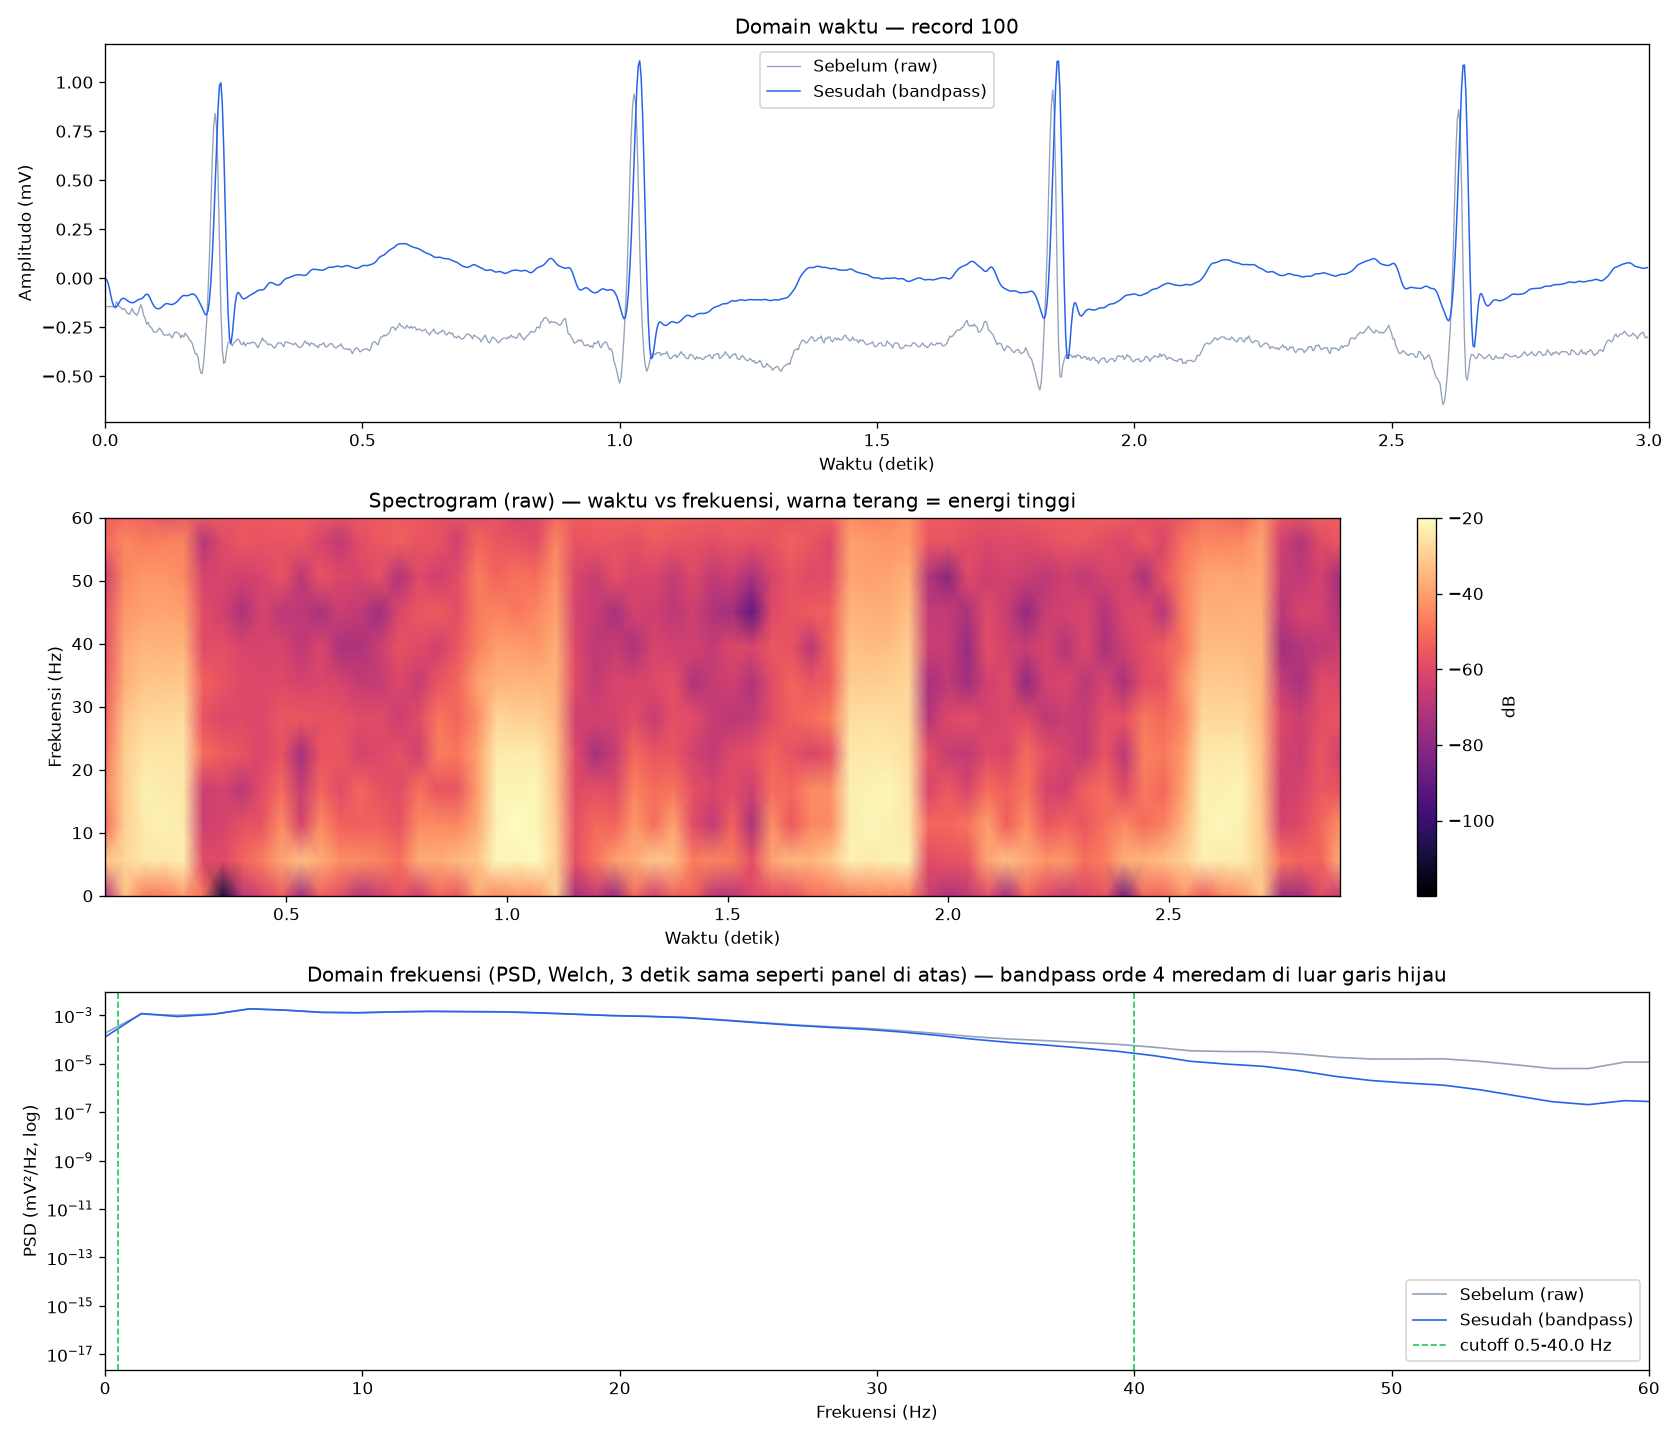
\includegraphics[width=\linewidth,height=0.5\textheight,keepaspectratio]{fase1_100.png}
  \caption{Sinyal rekaman 100 sebelum dan sesudah filter \textit{bandpass} kausal}
  \label{fig:hasil-filter}
\end{figure}

Gambar~\ref{fig:hasil-filter} terdiri atas tiga panel. Pada panel atas, filter memusatkan sinyal di sekitar nol, yaitu rata-rata berubah dari $-0{,}3063$ mV menjadi 0,0000 mV, sedangkan gelombang P, kompleks QRS, dan gelombang T tetap utuh. Simpangan baku sinyal hanya turun dari 0,1932 mV menjadi 0,1840 mV atau sekitar 4,8\%. Filter karena itu berperan sebagai pembersih dan bukan pemangkas morfologi. Puncak R pada sinyal tersaring tampak sedikit di kanan puncak pada sinyal mentah, yaitu \textit{group delay} sebesar 4 sampel atau sekitar 11 ms yang sengaja tidak dikoreksi. Panel tengah memperlihatkan spektrogram sinyal mentah dengan energi tertinggi mengumpul pada saat kompleks QRS dan pada frekuensi rendah. Pada panel bawah, kurva kerapatan spektral daya sesudah filter berimpit dengan kurva sebelum filter pada frekuensi rendah, lalu terpisah menjelang 40 Hz dan semakin jauh di bawahnya hingga 60 Hz.
% sumber: gambar laporan/buku-pa/gambar/fase1_100.png (dibuka dan dibaca); perhitungan ulang rekaman 100 (mean -0,3063 -> 0,0000, std 0,1932 -> 0,1840 = -4,8%); model/src/preprocessing.py design_bandpass_sos() (matriks 4 x 6, empat biquad); model/CLAUDE.md Fase 1 dan jebakan "Group delay filter kausal" (4 sampel / 360 Hz = 11,1 ms)

Hasil segmentasi \textit{window} 256 sampel beserta normalisasi \textit{z-score}, yang rancangannya ditunjukkan pada Gambar~\ref{fig:segmentasi}, diperiksa secara numerik pada rekaman 100. Sebanyak 2.273 anotasi menghasilkan 2.271 \textit{window} karena dua detak di tepi rekaman tidak memiliki cukup sampel. Setiap \textit{window} membentang 128 sampel atau sekitar 0,36 detik pada tiap sisi anotasi, dan seluruhnya berukuran 256 sampel dengan rata-rata mendekati nol serta simpangan baku 1,0000 setelah \textit{z-score}. Median indeks puncak R adalah 132 dan seluruh 2.271 \textit{window} memiliki puncak (nilai mutlak terbesar) dalam $\pm$2 sampel dari indeks tersebut.
% sumber: perhitungan ulang rekaman 100 dengan model/src/preprocessing.py segment_beats dan zscore_per_window (2.271 window, bentuk (2271, 256), median indeks puncak 132,0, seluruhnya dalam 132 +- 2, std z-score 1,0000); model/config.py (WIN_PRE 128, FS 360, 128/360 = 0,36 detik)

Ketiga tahap dinilai berjalan sesuai rancangan. Verifikasi ini hanya mencakup rekaman 100 dan 114. Pada rekaman 114, simpangan baku turun dari 0,3755 mV menjadi 0,3480 mV (7,3\%), seluruh 1.879 anotasi menghasilkan \textit{window}, dan 99,8\% \textit{window} memiliki puncak R dalam $\pm$2 sampel dari indeks 132.
% sumber: perhitungan ulang rekaman 114 (std 0,3755 -> 0,3480 = -7,3%, 1.879 window dengan 0 dibuang, 99,8% dalam 132 +- 2); model/CLAUDE.md Fase 1 (std 114 0,3755 -> 0,3480)

\subsubsection{Alur Hidup dan Beban Komputasi}

Seluruh rantai preprocessing harus berjalan secara \textit{real-time} di ESP32-S3 tanpa kehilangan sampel. Syaratnya adalah beban rata-rata per sampel lebih kecil daripada 2.778 $\mu$s atau 1/360 detik dan jumlah sampel yang hilang nol. Pengukuran memutar ulang sinyal acuan sampel demi sampel seolah-olah datang dari ADC pada 360 Hz, sedangkan waktu setiap panggilan pemrosesan dicatat dengan penghitung mikrodetik perangkat. Alur hidup yang diuji dimulai dari \textit{timer interrupt} atau \textit{interrupt service routine} (ISR) 360 Hz yang menaruh setiap sampel ke antrean 256 sampel. \textit{Loop} utama lalu menguras antrean dan memprosesnya sampai inferensi per detak, sebagaimana ditunjukkan pada Gambar~\ref{fig:alir-preprocessing}.
% sumber: firmware/test/test_inference/test_inference.cpp test_alur_hidup (anggaran 2778 us, micros(), golden_raw diputar per sampel); model/CLAUDE.md HW-3; firmware/src/akuisisi.cpp on_timer() dan loop(); firmware/include/ecg_live.h (ECG_LIVE_RING 4 * ECG_FS, ECG_LIVE_TIAP ECG_FS); model/docs/firmware-walkthrough.md bagian 5c

Hasil pengukuran ditunjukkan pada Tabel~\ref{tab:beban-komputasi}.

\begin{table}[!ht]
  \centering
  \caption{Beban komputasi dan antrean pada alur hidup}
  \label{tab:beban-komputasi}
  \setstretch{1.0}
  \setlength{\tabcolsep}{4pt}
  \renewcommand{\arraystretch}{1.15}
  \small
  \begin{tabularx}{\linewidth}{>{\RaggedRight\arraybackslash}X>{\raggedleft\arraybackslash}p{1.6cm}>{\RaggedRight\arraybackslash}X}
    \toprule
    \textbf{Besaran} & \textbf{Nilai} & \textbf{Kondisi Pengukuran} \\
    \midrule
    Anggaran waktu per sampel ($\mu$s) & 2.778 & 1/360 detik \\
    Beban rata-rata per sampel ($\mu$s) & 82 & \textit{Replay} sinyal acuan 2.400 sampel di perangkat, model \textit{window} 250 \\
    Puncak beban sesaat (ms) & 33,4 & Deteksi R-\textit{peak} dan inferensi bersamaan, model \textit{window} 250 \\
    Kapasitas antrean minimum menurut perhitungan (sampel) & 13 & Dihitung dari puncak beban sesaat \\
    Antrean saat puncak beban (sampel) & 12 & \textit{Firmware} produksi tanpa elektroda, ADC membaca derau, model \textit{window} 250 \\
    Antrean puncak (sampel) & 21 & \textit{Firmware} produksi dengan \textit{replay} sinyal acuan, model \textit{window} 256 \\
    Kapasitas antrean (sampel) & 256 & Antrean ISR pada kedua \textit{firmware} produksi \\
    Sampel hilang & 0 & Kedua pengukuran \textit{firmware} produksi \\
    \bottomrule
  \end{tabularx}
  \par\vspace{2pt}{\footnotesize\raggedright Keterangan: beban rata-rata setara 3,0\% anggaran dan puncak beban sesaat sekitar 12 kali anggaran. ISR adalah \textit{interrupt service routine}.\par}
\end{table}
% sumber: model/CLAUDE.md HW-3 (82 us/sampel dari 2778 us = 3,0%, burst 33,4 ms, antrean min 13), HW-4 (antrean 12 saat burst, sampel hilang 0), HW-7 Replay (antrean puncak 21/256, sampel hilang 0); model/docs/firmware-walkthrough.md bagian 5b dan 5c (burst 33.428 us, 12x anggaran satu sampel); 1/360 s = 2.777,8 us

Jalur preprocessing di perangkat tidak kehilangan sampel walaupun beban sesaatnya melampaui anggaran waktu (Tabel~\ref{tab:beban-komputasi}). Secara rata-rata pemrosesan hanya memakai 3,0\% anggaran per sampel. Beban itu menumpuk ketika deteksi R-\textit{peak} atas bufer empat detik bertepatan dengan inferensi detak baru, dan satu sampel dapat memakan sekitar 12 kali anggaran. Tanpa pembacaan ADC di ISR, setiap lonjakan seperti ini akan membuang sekitar 12 sampel dan merusak interval R-R. Antrean ISR menyerap lonjakan tersebut dengan terisi 12 sampel, mendekati kebutuhan 13 sampel hasil perhitungan dan jauh di bawah kapasitas 256 sampel atau sekitar 0,71 detik. Keluaran perangkat juga stabil, yaitu 11 detak per putaran \textit{replay} 6,67 detik atau sekitar 1,6 detak per detik, dengan pola probabilitas yang identik pada setiap putaran.
% sumber: model/CLAUDE.md HW-3, HW-4, HW-7 Replay (11 beat per putaran 6,67 detik, 11 / 6,67 = 1,65 beat/detik, pola p identik tiap putaran); model/CLAUDE.md jebakan "Beban alur hidup bursty" dan "Menunggu jaringan di dalam loop" (antrean 256 sampel @360 Hz = 711 ms); 256 / 360 = 0,711 detik

Pada pengujian \textit{replay} ditemukan satu kegagalan yang tidak langsung terlihat. Konversi nilai sinyal acuan dari \textit{float} ke \textit{count} ADC di dalam ISR membuat \textit{board} mengalami \textit{panic} bertipe \textit{coprocessor exception} pada detik ke-18,49, jadi lolos pada uji singkat. Penyebabnya, ESP32 tidak menyimpan register FPU saat masuk ISR. Penanganannya adalah mengonversi seluruh sinyal acuan ke tabel bilangan bulat sekali di \textit{setup}, dengan tambahan pemakaian RAM dari 21,2\% menjadi 22,7\% untuk tabel sebesar 4.800 byte. \textit{Board} yang me-\textit{reset} diam-diam membuat \textit{replay} nonaktif dan pengukuran melaporkan derau ADC. Status \textit{replay} karena itu diverifikasi dari ayunan sinyal.
% sumber: model/CLAUDE.md jebakan "Float di dalam ISR membunuh ESP32" (EXCCAUSE 0x00000004, detik 18, sim_counts); model/docs/firmware-walkthrough.md (panic di detik 18,49, RAM 21,2% -> 22,7%, sim_counts 4.800 byte); firmware/src/akuisisi.cpp (sim_counts dan on_timer)

Alur hidup dinilai memenuhi syarat \textit{real-time} pada sinyal \textit{replay}, yaitu beban rata-rata jauh di bawah anggaran dan sampel hilang nol. Beban rata-rata 82 $\mu$s dan puncak 33,4 ms diukur pada versi model \textit{window} 250 dan belum diukur ulang pada \textit{window} 256. Antrean puncak pada \textit{window} 256 tercatat 21 sampel, lebih tinggi daripada 12 sampel pada versi lama dan setara dengan sekitar 58 ms sampel yang tertahan. Kenaikan ini tidak dapat dijelaskan oleh pertambahan waktu inferensi per detak dari 26,0 ms menjadi 26,6 ms dan penyebabnya belum ditelusuri. Meskipun demikian, 21 sampel baru sekitar 8\% kapasitas antrean 256 sampel dan sampel hilang tetap nol. Pengukuran ini belum mencakup sinyal tubuh dan belum mencakup beban saat WiFi dan MQTT aktif.
% sumber: model/CLAUDE.md HW-1 (26,6 ms per detak, dari 26,0), HW-3 (versi window 250), HW-4 (antrean 12 saat burst), HW-7 Replay (antrean puncak 21/256 pada window 256, sampel hilang 0); 21 / 360 = 0,0583 detik = 58 ms; 21 / 256 = 8,2%

\subsubsection{Uji Perangkat dan Integrasi di \textit{Board}}

Setiap komponen perangkat diuji fungsinya, dan jalur \textit{real-time} diperiksa tetap tidak kehilangan sampel ketika layar dan \textit{buzzer} ikut bekerja, mengikuti rencana pengujian perangkat keras. Seluruh rangkaian uji di \textit{board} dijalankan pada 13 Oktober 2026 dengan rangkaian berpeta pin PCB, dan hasilnya per rangkaian uji ditunjukkan pada Tabel~\ref{tab:uji-papan}.
% sumber: git log f6042b5 (2026-10-13, "board 29/29, native 23/23") dan 07a5a07 (2026-10-13, "board: 29/29 test perangkat, native 23/23"); firmware/README.md bagian Test (jumlah per suite)

\begin{table}[!ht]
  \centering
  \caption{Hasil rangkaian uji di ESP32-S3 pada 13 Oktober 2026}
  \label{tab:uji-papan}
  \setstretch{1.0}
  \setlength{\tabcolsep}{4pt}
  \renewcommand{\arraystretch}{1.15}
  \small
  \begin{tabular}{>{\RaggedRight\arraybackslash}p{3.0cm}>{\centering\arraybackslash}p{1.5cm}>{\RaggedRight\arraybackslash}p{6.6cm}>{\centering\arraybackslash}p{1.4cm}}
    \toprule
    \textbf{Rangkaian Uji} & \textbf{Kasus} & \textbf{Yang Diverifikasi} & \textbf{Hasil} \\
    \midrule
    Inferensi & 5 & Inferensi model INT8 di perangkat, latensi, dan \textit{tensor arena} & Lulus \\
    Integrasi & 5 & Jalur \textit{real-time} utuh dengan layar dan \textit{buzzer} aktif; sampel hilang 0, laju jantung dalam 3 bpm & Lulus \\
    Layar & 2 & Inisialisasi TFT dan transfer SPI satu layar penuh & Lulus \\
    ADC dan \textit{lead-off} & 2 & ADC terbaca dan pewaktu menghasilkan 360 sampel per detik & Lulus \\
    Tombol & 2 & Ketiga pin berlogika HIGH saat diam dan uji tombol berakhir tepat pada batas waktunya & Lulus \\
    \textit{Buzzer} & 1 & Pin tersambung ke pembangkit nada setelah SPI layar terpasang, diam pada logika HIGH & Lulus \\
    Jumlah & 17 & & 17 lulus \\
    \bottomrule
  \end{tabular}
\end{table}
% sumber: firmware/README.md tabel Test dan baris "board 29 (test_preproc 11, test_inference 5, test_hw_integrasi 5, test_hw_tft 2, test_hw_adc 2, test_hw_tombol 2, test_hw_buzzer 1, test_hw_ina219 1)"; jumlah RUN_TEST per suite di firmware/test/test_*/; firmware/test/test_hw_integrasi/ (n_lewat == 0, PUTARAN 3, HR beda <= 3 bpm, label sama PC); git log f6042b5 (board 29/29)

Seluruh 17 kasus pada Tabel~\ref{tab:uji-papan} lulus. Hasil terpenting adalah uji integrasi. Pengukuran beban pada Tabel~\ref{tab:beban-komputasi} belum mencakup layar dan \textit{buzzer}, sedangkan uji integrasi menunjukkan sampel hilang tetap nol ketika gelombang digambar dan bip dibunyikan selama tiga putaran sinyal acuan. Uji integrasi juga memeriksa laju jantung yang ditampilkan, yaitu berselisih paling banyak 3 bpm dari interval R-R anotasi. Cakupannya perlu dicatat. Uji otomatis tidak menilai bunyi \textit{buzzer}, warna layar, dan tekanan tombol sungguhan, karena hal tersebut memerlukan pengamatan manusia dan diperiksa melalui menu Tes perangkat yang hasilnya tidak dicatat sebagai berkas. Uji integrasi juga dijalankan tanpa WiFi dan MQTT, jadi beban radio pada jalur \textit{real-time} belum tercakup dalam hasil ini.

Penguncian sesi perekaman diuji terpisah dengan menyuntikkan tekanan tombol dan perintah melalui serial ke perangkat yang sedang berjalan. Tujuh skenario diuji, yaitu sebagai berikut.
\begin{enumerate}
  \item Menu terkunci saat merekam.
  \item Menu tetap terkunci saat dijeda.
  \item Perubahan sumber, mode daya, pelewatan kalibrasi, WiFi, dan \textit{broker} ditolak saat merekam.
  \item Perekaman ditolak saat sumber \textit{replay}.
  \item Perekaman ditolak saat menu terbuka.
  \item Jeda dan lanjut diakhiri penyimpanan.
  \item Menu dapat dibuka kembali sesudah rekaman disimpan.
\end{enumerate}
Ketujuh skenario lulus pada dua putaran dengan sampel hilang nol selama sesi perekaman.
% sumber: git log 5088bb6 (2026-10-13, kunci sesi rekam: uji_alur_rekam.py 7/7 LULUS 2 putaran, sampel hilang 0 selama sesi rekam, pio test esp32-s3 29/29, native 23/23); model/scripts/uji_alur_rekam.py (skenario a-g, tombol disuntik lewat serial t/T); git log f6042b5 (native 23/23); firmware/test/test_hw_integrasi/ (PUTARAN 3, TFT digambar dan buzzer dibunyikan di loop uji, tanpa WiFi); firmware/README.md ("Bunyi buzzer dan isi layar dinilai langsung", menu Tes perangkat); bab4 tab:beban-komputasi (diukur tanpa antarmuka)

\subsubsection{Segmentasi di Perangkat}

Di perangkat, posisi R-\textit{peak} berasal dari detektor Pan-Tompkins, bukan dari anotasi seperti pada pelatihan. Biaya perbedaan itu diukur sebagai jumlah detak yang terlewat dan besarnya pengaruh pada klasifikasi. Pengukuran memakai DS2 dengan rangkaian koreksi posisi yang sama dengan kode C, yaitu kompensasi 38 sampel, penyelarasan ke puncak sinyal dalam $\pm$25 sampel, dan pengurangan \textit{group delay} 4 sampel. Nilai 38 sampel adalah median selisih antara deteksi dan anotasi pada DS1 dengan simpangan baku 13 sampel, jadi DS2 hanya dipakai untuk mengukur dan tidak untuk memilih parameter. Angka klasifikasi diukur pada model akhir versi \textit{float32}, yaitu \textit{window} 256 sampel dan \textit{threshold} 0,80, dan pada model acuan berukuran \textit{window} 250 sampel dengan \textit{threshold} 0,35 sebagai pembanding. Angka \textit{sensitivity} detektor tidak melibatkan model.
% sumber: model/docs/segmentasi-deteksi-walkthrough.md §1 dan §3 (offset median 38 sampel dikalibrasi di DS1; dua model: baseline window 90/160 threshold 0,35 dan model berlaku window 128/128 threshold 0,80, diukur ulang 13 Okt 2026 dengan model/scripts/eval_detected_segmentation.py); model/CLAUDE.md decision "Segmentasi on-device" (std 13 sampel); firmware/include/ecg_preproc.h (ECG_PT_OFFSET 38, ECG_PT_REFINE 25, ECG_GROUP_DELAY 4)

Keluaran detektor jatuh di sebelah kanan anotasi pasangannya, yaitu pada garis dasar sesudah kompleks QRS dan bukan pada puncak R. Pada sepuluh detik pertama rekaman 100, seluruh 13 anotasi memiliki 13 deteksi pasangan tanpa deteksi yang terlewat maupun berlebih. Pada keseluruhan rekaman 100, median selisih posisi adalah 40 sampel atau sekitar 0,11 detik, sejalan dengan median 38 sampel dari DS1. Keterlambatan ini sistematis dan karena itu dapat dikompensasi dengan satu konstanta, sedangkan penyelarasan ke puncak sinyal menyerap sisa variasinya.
% sumber: perhitungan ulang rekaman 100 dengan model/src/preprocessing.py pan_tompkins_detect (13 anotasi dan 13 deteksi pada 10 detik pertama, median selisih 40 sampel, std 12,1 sampel, 99,9% dalam 38 +- 25; 40/360 = 0,11 detik)

Detektor tidak melewatkan detak dengan peluang yang sama pada semua kelas, sebagaimana ditunjukkan pada Tabel~\ref{tab:sensitivity-detektor}.

\begin{table}[!ht]
  \centering
  \caption{\textit{Sensitivity} detektor Pan-Tompkins per kelas AAMI pada DS2}
  \label{tab:sensitivity-detektor}
  \setstretch{1.0}
  \setlength{\tabcolsep}{4pt}
  \renewcommand{\arraystretch}{1.15}
  \small
  \begin{tabular}{>{\RaggedRight\arraybackslash}p{4.2cm}>{\RaggedRight\arraybackslash}p{4.6cm}>{\centering\arraybackslash}p{3.0cm}}
    \toprule
    \textbf{Kelas} & \textbf{Keterangan} & \textbf{\textit{Sensitivity}} \\
    \midrule
    N & Normal & 0,9614 \\
    S & Supraventrikular, datang prematur & 0,6494 \\
    V & Ventrikular & 0,9146 \\
    F & Fusi & 0,9820 \\
    S, V, F, dan Q gabungan & Seluruh aritmia & 0,8296 \\
    Seluruh detak & 47.074 terdeteksi dan 2.638 terlewat & 0,9469 \\
    \bottomrule
  \end{tabular}
  \par\vspace{2pt}{\footnotesize\raggedright Keterangan: deteksi dipasangkan dengan anotasi dalam jendela 150 ms. Detektor juga menghasilkan 2.194 deteksi tanpa pasangan anotasi, jadi \textit{positive predictivity} seluruh detak 0,9555.\par}
\end{table}
% sumber: model/src/evaluate.py pair_detected dan model/scripts/eval_detected_segmentation.py (TOLERANSI_MS = 150); model/docs/segmentasi-deteksi-walkthrough.md bagian 3 (2.194 deteksi palsu); 47.074 / (47.074 + 2.194) = 0,9555; QRS Se dan +P dengan jendela 150 ms mengikuti PhysioNet bxb (docs/2026-11-01-crosscheck-metrik-bab4/klasifikasi.md butir 12)
% sumber: model/docs/segmentasi-deteksi-walkthrough.md bagian 3 dan 4 (47.074 terdeteksi, 2.638 terlewat, sensitivity 0,9469; per kelas N 0,9614, S 0,6494, V 0,9146, F 0,9820, Normal vs Aritmia 0,9614 vs 0,8296); model/scripts/eval_detected_segmentation.py (aritmia = S V F Q); diukur dengan detektor yang sama sebelum window dikunci 256, perhitungannya hanya dari pasangan deteksi dan anotasi sehingga tidak melibatkan model

Detektor menemukan 96,14\% detak Normal tetapi hanya 82,96\% detak aritmia (Tabel~\ref{tab:sensitivity-detektor}), dan kelas S menjadi yang paling sering terlewat dengan \textit{sensitivity} 0,6494. Penjelasan yang paling sesuai bersifat struktural. Detak supraventrikular datang prematur, sedangkan Pan-Tompkins menutup deteksi selama periode refraktori 200~ms sesudah detak sebelumnya, jadi detak yang datang terlalu cepat berpeluang terblokir. Penjelasan ini belum diuji dengan mengubah periode refraktori.
% sumber: model/docs/segmentasi-deteksi-walkthrough.md §4 (sebab struktural: beat S prematur terblokir periode refraktori 200 ms, PT_REFRACTORY_MS di model/config.py; trade-off refraktori belum diukur)

Dampak segmentasi hasil detektor terhadap klasifikasi ditunjukkan pada Tabel~\ref{tab:segmentasi-deteksi}. \textit{Recall} sistem memakai penyebut seluruh detak aritmia asli, termasuk yang tidak pernah terdeteksi, sedangkan \textit{recall}, \textit{precision}, dan F1 lainnya dihitung pada detak yang terdeteksi.

\begin{table}[!ht]
  \centering
  \caption{Klasifikasi DS2 model \textit{float32} dengan segmentasi anotasi dan segmentasi hasil detektor}
  \label{tab:segmentasi-deteksi}
  \setstretch{1.0}
  \setlength{\tabcolsep}{4pt}
  \renewcommand{\arraystretch}{1.15}
  \small
  \begin{tabular}{>{\RaggedRight\arraybackslash}p{3.0cm}>{\centering\arraybackslash}p{2.2cm}>{\centering\arraybackslash}p{2.2cm}>{\centering\arraybackslash}p{2.2cm}>{\centering\arraybackslash}p{2.2cm}}
    \toprule
    \textbf{Metrik} & \textbf{Acuan, anotasi} & \textbf{Acuan, detektor} & \textbf{Akhir, anotasi} & \textbf{Akhir, detektor} \\
    \midrule
    \textit{Recall} & 0,6661 & 0,6821 & 0,6996 & 0,7279 \\
    \textit{Precision} & 0,4919 & 0,4794 & 0,6235 & 0,5869 \\
    F1 & 0,5659 & 0,5631 & 0,6594 & 0,6499 \\
    \textit{Recall} sistem & 0,6661 & 0,5656 & 0,6996 & 0,6035 \\
    \bottomrule
  \end{tabular}
\end{table}
% sumber: model/docs/segmentasi-deteksi-walkthrough.md §3 tabel A (recall, precision, F1 baseline anotasi/deteksi dan berlaku anotasi/deteksi) dan blok B (recall sistem: baseline 3.084 / 5.453 = 0,5656, berlaku 3.291 / 5.453 = 0,6035); model/artifacts/metrics/fase6b_segmentasi_deteksi.csv memuat baris model acuan (f1 0,565903 / 0,563082, recall_sistem 0,666055 / 0,565560)

Segmentasi di perangkat tidak merusak klasifikasi selama ketiga koreksi posisi diterapkan (Tabel~\ref{tab:segmentasi-deteksi}). F1 dengan segmentasi detektor berselisih kurang dari 0,01 dari F1 dengan segmentasi anotasi pada kedua model, yaitu 0,6499 dibandingkan 0,6594 pada model akhir \textit{float32}. \textit{Recall} sistem model akhir turun dari 0,6996 menjadi 0,6035, dan seluruh penurunan ini berasal dari detak yang tidak pernah sampai ke model.

Penurunan \textit{recall} sistem tersebut berarti hanya 3.291 dari 5.453 detak aritmia asli yang tertangkap detektor lalu dikenali model. Detektor juga menghasilkan 2.194 deteksi palsu, dan 50,4\% di antaranya diklasifikasi Aritmia oleh model akhir, menambah 1.106 alarm palsu.
% sumber: model/docs/segmentasi-deteksi-walkthrough.md §3 blok B dan C (berlaku: 3.291 dari 5.453 tertangkap; 2.194 deteksi palsu, 50,4% diklasifikasi Aritmia = 1.106 alarm palsu tambahan); 0,6996 - 0,6035 = 0,0961

Segmentasi di perangkat dengan demikian layak, dan biayanya terletak pada detektor, bukan pada model. Detektor melewatkan sekitar 5\% detak secara keseluruhan dan sekitar sepertiga detak kelas S, sedangkan klasifikasi pada detak yang terdeteksi setara dengan klasifikasi pada segmentasi anotasi. Ketergantungan model terhadap posisi R yang presisi ditangani dengan latihan ber-\textit{jitter} pada jalur model.
% sumber: tab:sensitivity-detektor (sensitivity seluruh detak 0,9469, S 0,6494), tab:segmentasi-deteksi; model/docs/jitter-walkthrough.md (latih ulang dengan jitter)

\subsubsection{Akuisisi Sinyal Tubuh}

Sinyal tubuh dari modul AD8232 dinilai kelayakannya sebagai masukan jalur preprocessing. Rekaman diambil dengan konfigurasi Lead II, elektroda \textit{wet-gel}, dan daya dari \textit{powerbank} agar perangkat tidak tersambung ke jala-jala selama perekaman. Setiap rekaman dilaporkan dengan empat ukuran, yaitu ayunan sinyal ADC absolut, persentase dengung 50 Hz terhadap energi pita ECG 0,5--40 Hz~\cite{gajdzik_2026}, jumlah R-\textit{peak} yang ditemukan Pan-Tompkins, dan jumlah sampel jenuh. Kelayakan rekaman dinilai dengan indeks kualitas sinyal per jendela 10 detik. Pada rekaman yang dijeda, R-\textit{peak} dan interval R-R dihitung per segmen agar tidak ada interval R-R yang melintasi jeda.

Ayunan dalam mV dihitung sebagai ekuivalen masukan AD8232, yaitu jumlah \textit{count} dikalikan 0,757 mV per \textit{count} dari ADC 12-bit dengan atenuasi 11 dB, lalu dibagi \textit{gain} AD8232 sekitar 1.100. Dengan konversi ini, ECG sehat berayun sekitar 2 mV atau sekitar 3.000 \textit{count}, sedangkan ayunan di bawah sekitar 0,1 mV atau 150 \textit{count} berarti tidak ada biopotensial sama sekali.

Ayunan, dengung, dan sampel jenuh dilaporkan tanpa ambang lulus, karena acuan baku untuk ambang ketiganya tidak ditemukan. Definisi rasio dengung mengikuti penelitian yang membandingkan jalur akuisisi AD8232 dengan ADC 12-bit ESP32, yang juga tidak menetapkan ambang lulus~\cite{gajdzik_2026}. Sampel jenuh adalah sampel di batas atas atau bawah ADC. Gerbang kualitas waktu nyata, yaitu kontak elektroda dan interval R-R, dipakai sebelum detak diteruskan dan diuji tersendiri dengan sinyal tubuh.
% sumber: model/CLAUDE.md jebakan "Telemetri akuisisi bisa berbohong" (konversi 12-bit + atten 11 dB = 0,757 mV/count, gain AD8232 sekitar 1100, EKG sehat sekitar 2 mV sekitar 3000 count, di bawah sekitar 0,1 mV sekitar 150 count tidak ada biopotensial); model/docs/akuisisi-walkthrough.md bagian 1 (USB laptop vs power bank) dan bagian 6 (ukuran dan ambang); firmware/src/perangkat.cpp (ADC_WIDTH_BIT_12, ADC_ATTEN_DB_12, nama lain atenuasi 11 dB); model/scripts/analyze_recording.py (masuk_akal 30-200 bpm; muat() dan analisis_segmen() memisah segmen pada baris jeda)
% sumber: keputusan user 1 Nov 2026 (ambang tanpa rujukan dihapus: dengung < 15%, autokorelasi > 0,25, BPM wajar > 90%, jenuh 0,1%, status Berhasil/Bersinyal/Gagal; diganti indeks kualitas per jendela 10 detik); Gajdzik dkk. 2026 hlm. 59-63 (PLIratio tanpa ambang lulus); rail jenuh ADC_ATAS 4090 dan ADC_BAWAH 5 dari model/scripts/analyze_recording.py hitung_clipping(); gerbang waktu nyata dari bab3.tex gerbang kualitas

Kelayakan setiap rekaman dinilai per jendela 10 detik dengan indeks kualitas sinyal empat langkah~\cite{syversen_2024}, jadi bagian rekaman yang buruk tidak tersembunyi oleh nilai keseluruhan. Tiga langkah pertama memeriksa kelayakan fisiologis, yaitu detak per menit 40 sampai 180, jeda antar-R-\textit{peak} paling lama 3 detik, dan rasio interval R-R terpanjang terhadap terpendek di bawah 2,2. Langkah keempat memotong setiap kompleks QRS selebar median interval R-R dan merata-ratakannya menjadi \textit{template}. Jendela dinyatakan lolos bila rerata korelasi setiap potongan terhadap \textit{template} minimal 0,66. Hasil pengujian rekaman resmi ditunjukkan pada Tabel~\ref{tab:kualitas-rekaman}.
% sumber: Syversen dkk. 2024 bagian SQI1 ("HR-check of 40 and <180 bpm, ... maximum space between subsequent R-peaks is <3 s ... ratio is <2.2 ... adaptive template matching threshold (0.66)"), metode asli Orphanidou dkk. 2015 hlm. 834-836 (potongan selebar median RR berpusat di R); model/scripts/kualitas_jendela.py; model/docs/akuisisi-walkthrough.md bagian 6 SQI per jendela 10 detik

\begin{table}[!ht]
  \centering
  \caption{Kualitas rekaman AD8232 pada pengujian rekaman resmi}
  \label{tab:kualitas-rekaman}
  \setstretch{1.0}
  \setlength{\tabcolsep}{2.5pt}
  \renewcommand{\arraystretch}{1.15}
  \footnotesize
  \begin{tabular}{>{\centering\arraybackslash}p{1.5cm}>{\raggedleft\arraybackslash}p{1.1cm}>{\centering\arraybackslash}p{1.8cm}>{\raggedleft\arraybackslash}p{1.4cm}>{\raggedleft\arraybackslash}p{1.1cm}>{\raggedleft\arraybackslash}p{1.0cm}>{\raggedleft\arraybackslash}p{1.2cm}>{\raggedleft\arraybackslash}p{1.3cm}>{\raggedleft\arraybackslash}p{1.5cm}}
    \toprule
    \textbf{Rekaman} & \textbf{Durasi (detik)} & \textbf{Ayunan (\textit{count} / mV)} & \textbf{Dengung (\%)} & \textbf{R-\textit{peak}} & \textbf{Jenuh} & \textbf{Jendela} & \textbf{Jendela Lolos (\%)} & \textbf{Korelasi Mini\-mum} \\
    \midrule
    \multicolumn{9}{l}{\textit{Sesi 22 Oktober 2026, subjek S01, Lead II, catu powerbank}} \\
    R1 & 300,0 & 2.928 / 2,01 & 1,9 & 402 & 1 & 30 & 100,0 & 0,981 \\
    R2 & 300,0 & 3.012 / 2,07 & 3,1 & 408 & 5 & 30 & 100,0 & 0,967 \\
    R3 & 300,0 & 3.104 / 2,14 & 2,9 & 425 & 9 & 30 & 100,0 & 0,967 \\
    R4 & 27,1 & 2.919 / 2,01 & 3,8 & 40 & 1 & 2 & 100,0 & 0,980 \\
    \bottomrule
  \end{tabular}
  \par\vspace{2pt}{\footnotesize\raggedright Keterangan: R1 sampai R4 adalah empat rekaman berurutan dari satu sesi tanpa jeda. Jenuh adalah jumlah sampel di batas ADC, paling banyak 0,010\% sampel rekaman. Jendela adalah jumlah jendela 10 detik utuh. Korelasi minimum adalah rerata korelasi \textit{template} terendah di antara jendela rekaman. Status \textit{lead-off} 0\% pada keempat rekaman.\par}
\end{table}
% sumber: jendela, jendela lolos, dan korelasi minimum dari model/scripts/kualitas_jendela.py -> model/artifacts/metrics/kualitas/jendela10s_20261022-*.csv (30/30/30/2 jendela, 100% lolos, korelasi minimum 0,981, 0,967, 0,967, 0,980)
% sumber: keluaran make analisis FILE=data/recordings/<nama>.csv pada 20261022-1256-rekam-001 (ADC 1167..4095, dengung 1,9%, autokorelasi 0,37 median per 30 s, R-peak 402 dalam 300,0 detik, masuk akal 100%), -1256-rekam-002 (1083..4095, 3,1%, 0,38, 408), -1257-rekam-003 (991..4095, 2,9%, 0,33, 425), -1257-rekam-004 (1176..4095, 3,8%, 0,28 tanpa jendela, 40 dalam 27,1 detik); ayunan = maks - min (2.928, 3.012, 3.104, 2.919), mV = count x 0,757 / 1100 (2,01, 2,07, 2,14, 2,01); jenuh dengan rail firmware 4090/5 = 1, 5, 9, 1 sampel (0,001%, 0,005%, 0,008%, 0,010%); header lepas=0 (0%) pada keempat berkas; rekaman uji coba 10 Sep - 11 Okt 2026 tidak dimasukkan (arsip model/data/arsip/rekaman-uji-coba/, bukan hasil)

Keempat rekaman resmi lolos indeks kualitas sinyal pada seluruh jendela 10 detik (Tabel~\ref{tab:kualitas-rekaman}). Korelasi \textit{template} terendah 0,967, jauh di atas batas 0,66, dan ayunan sekitar 2 mV sesuai dengan ECG sehat. Dengung paling besar 3,8\%, dan sampel jenuh hanya muncul sesekali pada puncak R. Penilai yang sama menolak seluruh jendela rekaman uji coba yang hanya berisi derau, jadi kelolosan ini bukan akibat syarat yang terlalu longgar. Sinyal tubuh pada sesi ini karena itu layak dijadikan masukan jalur preprocessing.
% sumber: tab:kualitas-rekaman (92 jendela lolos 100%, korelasi minimum 0,967 pada R2 dan R3; dengung maksimum 3,8% pada R4; ayunan 2,01-2,14 mV; jenuh maksimum 1 dari 9.771 = 0,010%); kontrol negatif rekaman uji coba arsip berayun 16-55 count lolos 0% jendela (model/docs/akuisisi-walkthrough.md bagian 6)

Bentuk sinyal rekaman yang berhasil ditunjukkan pada Gambar~\ref{fig:rekaman-berhasil}, yaitu enam detik pertama rekaman R1.

\begin{figure}[!ht]
  \centering
  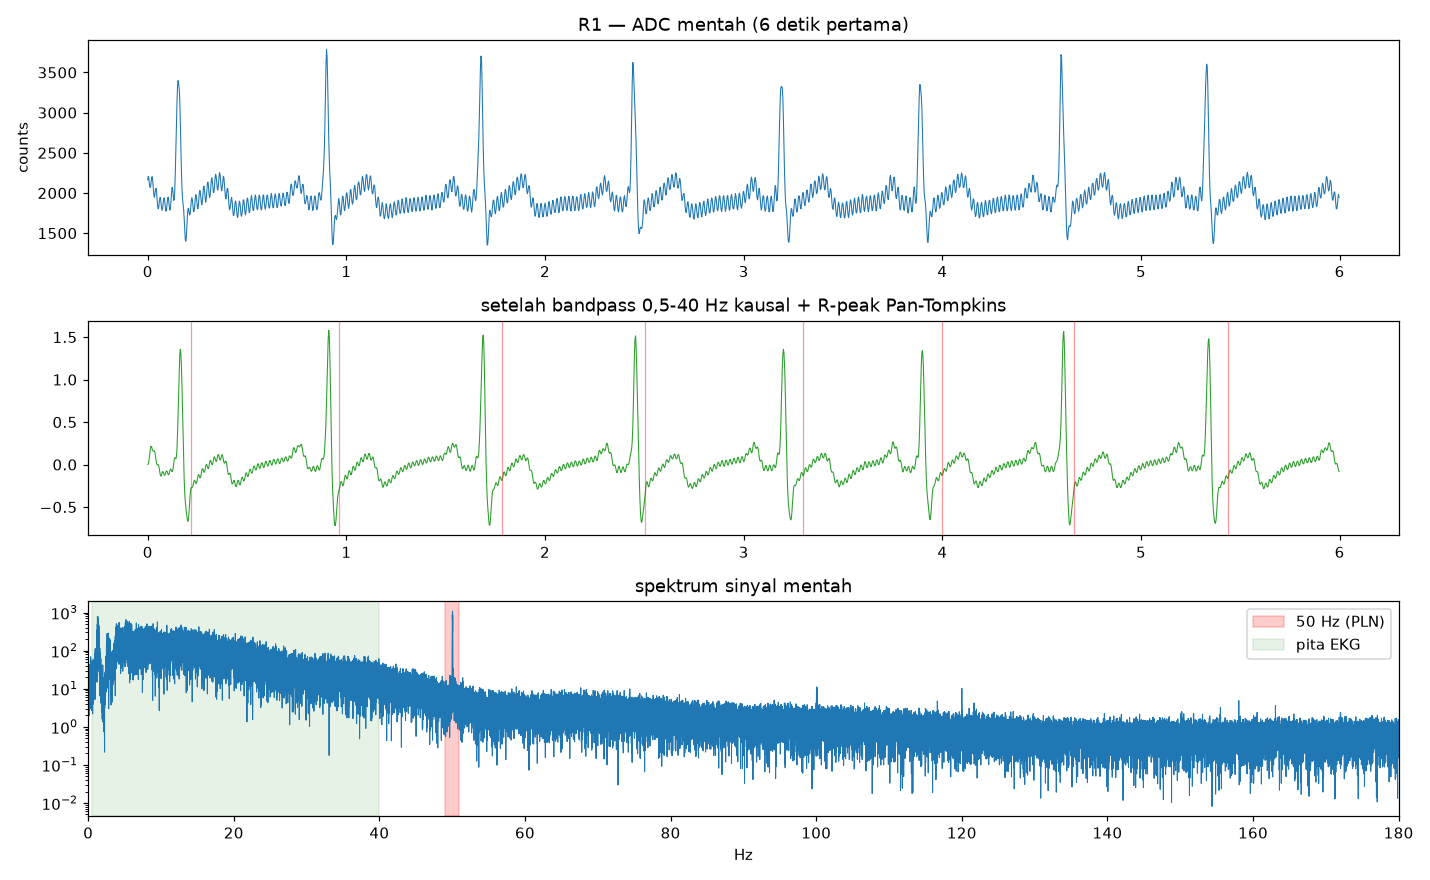
\includegraphics[width=\linewidth,height=0.45\textheight,keepaspectratio]{akuisisi_20261022-1256-rekam-001.png}
  \caption{Rekaman AD8232 yang berhasil, enam detik pertama rekaman R1}
  \label{fig:rekaman-berhasil}
\end{figure}
% sumber: model/artifacts/metrics/akuisisi/akuisisi_20261022-1256-rekam-001.png (make analisis), disalin ke laporan/buku-pa/gambar oleh scripts/export_artifacts.sh --laporan

Gambar~\ref{fig:rekaman-berhasil} terdiri atas tiga panel. Panel pertama menampilkan ADC mentah, dan panel kedua sinyal sesudah \textit{bandpass} dengan garis merah pada setiap R-\textit{peak} hasil Pan-Tompkins. Panel ketiga menampilkan spektrum dengan pita merah untuk dengung 50 Hz serta pita hijau untuk pita ECG. Pada panel pertama, puncak QRS mencapai sekitar 3.300 sampai 3.800 \textit{count} di atas garis dasar sekitar 1.900 \textit{count}. Panel kedua memuat delapan R-\textit{peak} dengan jarak antarpuncak sekitar 0,7 sampai 0,8 detik. Panel ketiga memperlihatkan puncak sempit pada 50 Hz di luar pita ECG. Filter \textit{bandpass} hanya meredam 50 Hz sebesar 9,3 dB, yaitu penguatan 0,342, jadi dengung yang masuk ke ADC tetap tampak sebagai gerigi halus pada garis dasar panel kedua.
% sumber: dibaca dari model/artifacts/metrics/akuisisi/akuisisi_20261022-1256-rekam-001.png (puncak QRS 3.300-3.800 count, garis dasar sekitar 1.900, 8 garis R-peak dalam 6 detik, puncak 50 Hz pada spektrum)
% sumber: tiga panel dari model/scripts/analyze_recording.py (ADC mentah, bandpass + garis R-peak, spektrum pita 50 Hz merah dan pita EKG hijau; model/docs/akuisisi-walkthrough.md §5); model/docs/akuisisi-walkthrough.md §2 (bandpass meredam 50 Hz -9,3 dB, gain 0,342) dan perhitungan ulang sosfreqz atas model/src/preprocessing.py design_bandpass_sos() pada 50 Hz (gain 0,3422 = -9,31 dB)

Prosedur perekaman pada pengujian ini, yaitu catu daya \textit{powerbank}, elektroda baru yang ditempel sekali, dan penilaian kualitas dari ayunan ADC absolut, disusun dari perekaman uji coba selama pengembangan. Perekaman uji coba tersebut memakai rangkaian yang masih berubah sehingga tidak dilaporkan sebagai hasil.
% sumber: model/docs/akuisisi-walkthrough.md §1 (powerbank, elektroda sekali tempel), §6 (ayunan ADC absolut sebagai wasit) dan §8 (rekaman uji coba, arsip model/data/arsip/rekaman-uji-coba/)

Keberadaan R-\textit{peak} tidak dapat dijadikan penentu kualitas sinyal. Pan-Tompkins tetap melaporkan R-\textit{peak} karena ambangnya adaptif terhadap sinyal yang ada, dan keadaan tanpa sinyal bukan kondisi yang dikenalinya. Pada \textit{firmware}, tanpa elektroda dan tanpa \textit{replay}, alat mengeluarkan sekitar 2 detak per detik dengan 57\% di antaranya diklasifikasi Aritmia. Kualitas sinyal di perangkat karena itu dinilai dari kontak elektroda, yaitu status \textit{lead-off}, ayunan ADC, dan dengung 50 Hz.
% sumber: model/CLAUDE.md jebakan "Tanpa elektroda, alat mengarang aritmia: ~2 beat/detik, 57% ARITMIA" dan "Telemetri akuisisi bisa berbohong"; model/docs/akuisisi-walkthrough.md bagian 6

Hasil akuisisi tersebut adalah status fungsional, bukan akurasi. Jumlah R-\textit{peak} dan indeks kualitas sinyal menunjukkan bahwa detektor menemukan detak dengan irama yang masuk akal. Namun, posisi R-\textit{peak} dan detak per menit belum dibandingkan dengan perangkat ECG acuan maupun anotasi manual. Rentang masukan juga terbatas. Dengan garis dasar sekitar 1.900 \textit{count}, ruang sampai batas atas ADC hanya sekitar 1,5 mV ekuivalen masukan, dan karena itu puncak R sesekali terpotong. Filter 0,5--40 Hz yang kausal dipilih untuk analisis ritme dan klasifikasi detak, jadi rekaman ini tidak dimaksudkan untuk analisis segmen ST.
% sumber: keputusan user 1 Nov 2026 (hasil akuisisi ditulis sebagai status fungsional karena belum ada alat medis acuan); docs/2026-11-01-crosscheck-metrik-bab4.md bagian 4 dan akuisisi.md butir 1, 2, 9; ruang atas (4.095 - 1.900) x 0,757 / 1.100 = 1,51 mV dari garis dasar Gambar rekaman R1; model/config.py BANDPASS_LOW 0.5, BANDPASS_HIGH 40.0, filter kausal sosfilt

Dengan demikian, sinyal tubuh dari satu sesi perekaman layak secara fungsional sebagai masukan jalur preprocessing, dengan keempat rekamannya lolos indeks kualitas sinyal pada seluruh jendela, sehingga target akuisisi terpenuhi.
% sumber: tab:kualitas-rekaman (4 dari 4 Berhasil, satu sesi)

\subsubsection{Gerbang Kalibrasi dan Kualitas Sinyal}

Hanya detak dari sinyal layak yang boleh diteruskan ke antrean pengiriman. Gerbang kalibrasi, dengan alur penilaian pada Gambar~\ref{fig:alir-firmware}, menilai kontak elektroda setiap detik dari status \textit{lead-off}, ayunan bersih minimal 60 \textit{count}, dan dengung 50 Hz paling besar 500 \textit{count}. Fase kalibrasi berakhir setelah kontak baik bertahan 60 detik dan interval R-R memenuhi kriteria selama 30 detik. Sesudah itu kontak tetap dinilai setiap detik, dan detak ditahan selama kontak buruk.
% sumber: firmware/include/gerbang.h (AMBANG_AYUN 60, AMBANG_DENGUNG 500, PEMANASAN_MS 60 s, RR_TENANG_MS 30 s); firmware/src/gerbang.cpp nilai_kontak() (lepas, ayun_bersih, hum50; fase BAIK/BURUK tiap detik) dan gerbang_nilai_fase() (kontak 60 s && rr_tenang); model/docs/mqtt-walkthrough.md §3.1

Durasi 60 detik ditetapkan dari pengukuran waktu stabil pada tiga sesi perekaman sekitar 15 menit. Pada ketiga sesi, ayunan bersih sudah mencapai 60 \textit{count} sejak detik pertama, dan kriteria R-R terpenuhi pada detik ke-30. Dengung 50 Hz tidak memperlihatkan pola pemanasan yang sama antarsesi. Pada satu sesi, dengung melonjak bertahap hingga sekitar 2.800 \textit{count} saat kontak memburuk, sementara ayunan tetap di atas 1.400 \textit{count} dan interval R-R tetap wajar. Waktu tunggu tetap 10--15 menit karena itu tidak didukung pengukuran, dan ayunan saja tidak cukup untuk menilai kontak.
% sumber: model/scripts/tren_kualitas.py atas tiga sesi (model/artifacts/metrics/kualitas/20261021-1549-rekam-001-sesi6.csv, 20261022-1219-rekam-002-sesi4.csv, 20261022-1256-rekam-001-sesi4.csv): ayun_bersih >= 60 pertama 0 s, RR tenang >= 30 s pertama 30 s pada ketiganya; sesi 22 Okt pagi dengung per 10 s sampai 2.782 (810-840 s), ayun_bersih per menit >= 1.469, RR wajar 97,6-100%; model/data/recordings/README.md Catatan per sesi

Gerbang diuji dengan sinyal tubuh pada 22 Oktober 2026 dalam tiga keadaan. Dengan kontak elektroda yang buruk, status \textit{lead-off} menandai elektroda lepas pada setiap detik selama sekitar empat menit, dan ayunan hanya naik hingga sekitar 395 \textit{count}. Fase kalibrasi tidak berakhir walaupun ayunan sesekali melampaui 60 \textit{count}. Dengan elektroda baru dan catu \textit{powerbank}, bip panjang dan LED hijau muncul sekitar 60 detik setelah elektroda menempel, lalu bip detak mulai berbunyi. Klip kabel LA yang dicabut sekitar 10 detik mengubah LED menjadi oranye, dan LED kembali hijau tanpa menunggu 60 detik setelah klip dipasang lagi.
% sumber: model/docs/mqtt-walkthrough.md §3.1c (uji gerbang kontak 22 Okt 2026): langkah 2 log serial 13:09:46-13:13:41 (lepas 1, kontak 0/60 s, ayun 11-395); langkah 3 diamati subjek di layar dengan catu powerbank, tanpa log serial

Pada sumber sinyal \textit{replay}, syarat lama kontak, syarat R-R, dan status \textit{lead-off} dilewati. Potongan 6,67 detik dari rekaman 208 bersifat aritmik dengan selisih R-R antardetak hingga $-$0,364 dan $+$0,478 detik, dan kriteria R-R tidak akan terpenuhi. Pelewatan tersebut melekat pada sumber \textit{replay}. Pada uji 22 Oktober 2026, sumber yang dikembalikan ke sensor tanpa elektroda tetap berada pada fase kalibrasi dengan ayunan 1 \textit{count}. Pada pengujian awal tanpa elektroda, 19 detak terdeteksi dengan tujuh di antaranya diklasifikasi Aritmia, dan seluruhnya ditahan sehingga tidak satu pun terkirim ke \textit{broker}.
% sumber: model/docs/mqtt-walkthrough.md §3.1b (dRR rekaman 208 -0,364 s dan +0,478 s), §3.1c langkah 1 (replay ON lolos dengan LO 1 1; replay OFF tanpa elektroda: calibrating, ayun 1) dan bagian "Jalur data, terukur" (tanpa elektroda: beat 19 (7 aritmia, 19 ditahan), terkirim 0); firmware/src/gerbang.cpp nilai_kontak() (LO diabaikan saat akuisisi_replay())

Uji tersebut menunjukkan bahwa gerbang menahan sinyal tanpa elektroda dan kontak yang buruk, lalu membuka pemantauan sekitar 60 detik setelah kontak baik pada satu subjek. Transisi pada kontak baik diamati langsung pada perangkat karena serial tidak tersambung selama catu \textit{powerbank}, dan belum tercatat sebagai log. Gerbang kalibrasi karena itu berfungsi sesuai rancangan pada sinyal tubuh satu subjek.

\subsection{Jalur Model TinyML \textit{On-Device}}

Model TinyML terkuantisasi INT8 diterapkan untuk deteksi aritmia secara \textit{on-device} pada ESP32-S3 tanpa ketergantungan pada komputasi \textit{cloud}. Targetnya mengikuti Tabel~\ref{tab:pengujian-model}. Target itu mencakup kualitas klasifikasi DS2 pada \textit{threshold} hasil kalibrasi VAL dan F1 model INT8 minimal 99\% F1 \textit{float32}. Target lainnya adalah latensi di bawah interval antardetak dan model yang muat di memori. Hasilnya dipaparkan dalam enam butir berikut.
% sumber: laporan/buku-pa/bab/bab1.tex Tujuan butir 2; laporan/buku-pa/bab/bab3.tex tab:pengujian-model (|delta recall| < 0,02, ukuran < 25 KB, latensi < interval antardetak, daya per mode operasi)

\subsubsection{Pelatihan dan Pemilihan Titik Operasi}

Model dan titik operasinya diperoleh dengan \textit{epoch} dan \textit{threshold} yang ditentukan hanya dari VAL. Model \textit{hybrid} dengan 6.417 parameter dilatih pada 121.857 baris DS1, yaitu 40.619 detak beserta dua salinan ber-\textit{jitter}. VAL sebanyak 31.047 baris dipakai untuk \textit{early stopping} dan kalibrasi \textit{threshold}. Perjalanan pelatihan ditunjukkan pada Gambar~\ref{fig:hasil-latih}.
% sumber: laporan/buku-pa/bab/bab4.tex tab:dataset (DS1 latih 121.857 = 40.619 x 3, VAL 31.047, 6.417 parameter); model/config.py (BATCH_SIZE 64, EARLY_STOP_PATIENCE 8, EARLY_STOP_MONITOR val_auc)

\begin{figure}[H]
  \centering
  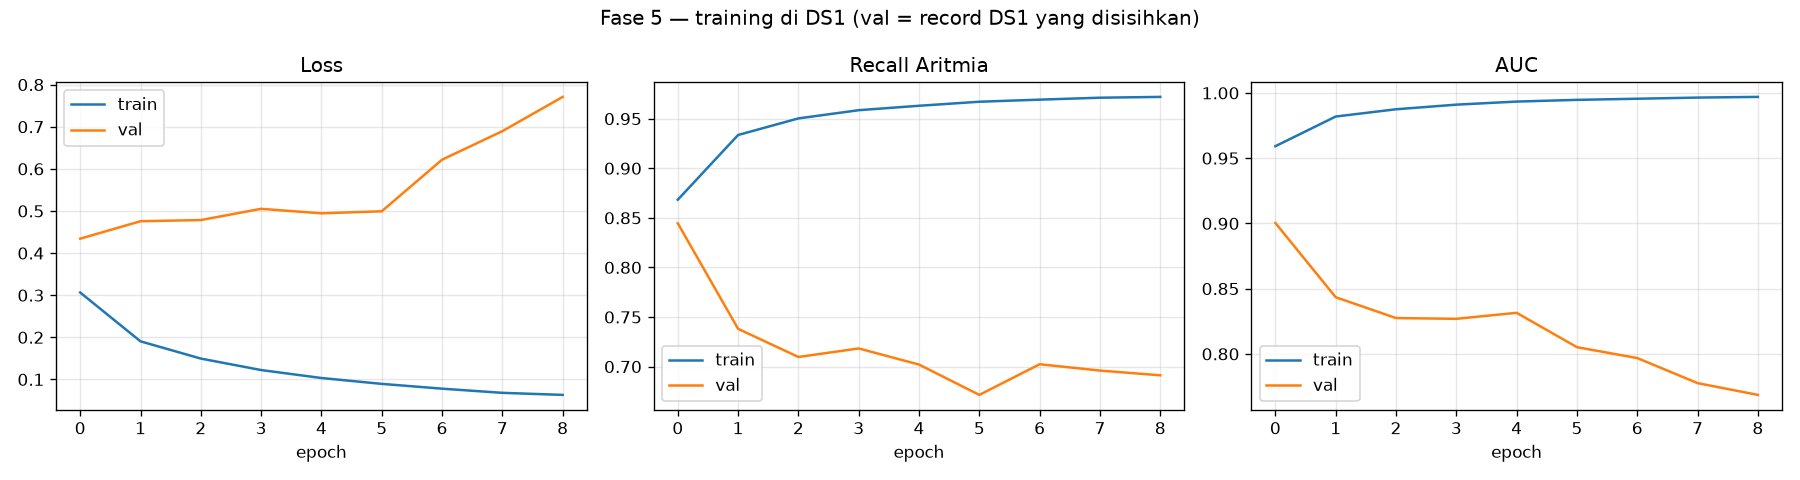
\includegraphics[width=\linewidth,keepaspectratio]{fase5_training.png}
  \caption{Kurva \textit{loss}, \textit{recall} Aritmia, dan AUC selama pelatihan model pada DS1}
  \label{fig:hasil-latih}
\end{figure}

Gambar~\ref{fig:hasil-latih} memperlihatkan kurva data latih berwarna biru yang terus membaik, sedangkan kurva VAL memburuk sejak \textit{epoch} pertama. Pada kurva VAL berwarna jingga, \textit{loss} naik dari sekitar 0,43 menjadi sekitar 0,77, dan \textit{recall} pada \textit{threshold} bawaan 0,5 turun dari sekitar 0,85 menjadi sekitar 0,69. AUC validasi memuncak sekitar 0,90 pada \textit{epoch} 0, yaitu \textit{epoch} pertama karena penomoran dimulai dari nol, lalu turun hingga sekitar 0,77 pada \textit{epoch} 8. Karena AUC validasi tidak pernah melampaui nilai \textit{epoch} 0, \textit{early stopping} mengembalikan bobot \textit{epoch} 0, dan model yang dipakai adalah hasil satu \textit{epoch} pelatihan. Penyebabnya diduga jumlah langkah gradien, karena augmentasi tiga salinan membuat satu \textit{epoch} berisi 1.905 langkah, yaitu 121.857 baris dibagi ukuran \textit{batch} 64, yang sudah cukup bagi 6.417 parameter untuk menyesuaikan diri dengan data latih.

\textit{Threshold} kemudian dipilih dari \textit{sweep} 0,05 sampai 0,95 pada VAL dengan kriteria F1 maksimum dan \textit{recall} sebagai penentu bila selisih F1 kurang dari 0,005. Nilai 0,80 memberi F1 VAL tertinggi sebesar 0,6917 dan 0,85 memberi 0,6886 dengan selisih kurang dari 0,005. Keduanya karena itu dibandingkan dengan \textit{recall}, dan 0,80 menang dengan 0,6539 dibandingkan 0,6141.
% sumber: gambar laporan/buku-pa/gambar/fase5_training.png (dibuka dan dibaca, sumbu epoch 0 sampai 8, biru = train, jingga = val; val loss 0,43 ke 0,77, val recall 0,85 ke 0,69, val AUC 0,90 ke 0,77); model/src/train.py (metrics.Recall dengan threshold bawaan 0,5, EarlyStopping restore_best_weights); model/docs/arsip/2026-09-19-faseG-changelog.md bagian 2 (1.905 langkah gradien per epoch, val_auc memuncak di epoch 0); 121.857 / 64 = 1.904,02 sehingga 1.905 langkah
% sumber: model/scripts/calibrate_threshold.py (sapuan 0,05-0,95 langkah 0,05, F1_TIE_MARGIN 0,005, pilih recall tertinggi di antara kandidat); model/artifacts/metrics/fase5_threshold_sweep.csv (0,80: f1 0,691724 recall 0,653920; 0,85: f1 0,688583 recall 0,614085); model/config.py THRESHOLD = 0.80

\subsubsection{Evaluasi pada DS2}

Kemampuan model diukur pada pasien yang tidak pernah dilihat saat pelatihan. Model INT8 yang dijalankan di perangkat dievaluasi pada 49.656 detak DS2 dari 22 pasien, termasuk 5.450 detak Aritmia, pada \textit{threshold} 0,80 dengan metrik pada Persamaan~\ref{eq:metrik}. Seluruh detak setiap rekaman dipakai, termasuk lima menit pertama yang pada protokol evaluasi AAMI dikecualikan sebagai periode belajar~\cite{aami_ec57_2012}. Periode belajar tidak relevan karena model tidak beradaptasi per pasien, dan pembagian \textit{inter-patient} de Chazal juga memakai rekaman penuh~\cite{dechazal_2004}. Hasilnya ditunjukkan pada Tabel~\ref{tab:hasil-ds2}, sedangkan model \textit{float32} dipakai sebagai pembanding kuantisasi.
% sumber: model/artifacts/metrics/fase6_per_record_fp32.csv (22 rekaman, jumlah n_beat 49.656, jumlah n_aritmia 5.450); model/scripts/eval_fp32.py (threshold dari config.THRESHOLD, tidak disetel di DS2)
% sumber: periode belajar 5 menit dari PhysioNet WAG "Evaluating ECG Analyzers" dan bxb (default -f 5 menit, mengacu EC38/EC57); de Chazal 2004 dan Luz 2016 Tabel 6 memakai seluruh detak DS2; docs/2026-11-01-crosscheck-metrik-bab4/klasifikasi.md butir 4

\begin{table}[!ht]
  \centering
  \caption{Hasil klasifikasi model INT8 pada DS2 dengan \textit{threshold} 0,80}
  \label{tab:hasil-ds2}
  \setstretch{1.0}
  \setlength{\tabcolsep}{4pt}
  \renewcommand{\arraystretch}{1.15}
  \small
  \begin{tabular}{>{\RaggedRight\arraybackslash}p{4.4cm}>{\raggedleft\arraybackslash}p{2.2cm}}
    \toprule
    \textbf{Metrik} & \textbf{Nilai} \\
    \midrule
    \textit{Recall} & 0,7105 \\
    \textit{Precision} & 0,6169 \\
    F1 & 0,6604 \\
    \textit{Specificity} & 0,9456 \\
    MCC & 0,6171 \\
    AUC & 0,9344 \\
    \textit{Accuracy} & 0,9198 \\
    \bottomrule
  \end{tabular}
  \par\vspace{2pt}{\footnotesize\raggedright Keterangan: TP 3.872, FN 1.578, FP 2.405, dan TN 41.801 dari 5.450 detak Aritmia dan 44.206 detak Normal. \textit{Accuracy} dilaporkan tetapi bukan acuan.\par}
\end{table}
% sumber: model/artifacts/metrics/fase6_metrics_fp32.csv (threshold 0.80, tp 3813, fn 1637, fp 2302, tn 41904, accuracy 0,920674, precision 0,623549, recall 0,699633, specificity 0,947926, f1 0,659403, auc 0,933448); 41.904 + 2.302 = 44.206 detak Normal; MCC 0,615986 dari model/artifacts/metrics/fase7_metrik_tambahan.csv (model/scripts/metrik_tambahan.py)

Model INT8 menemukan sekitar tujuh dari sepuluh detak Aritmia pada pasien yang tidak pernah dilihat saat pelatihan (Tabel~\ref{tab:hasil-ds2}). \textit{Recall} 0,7105 dicapai dengan \textit{precision} 0,6169, yang berarti sekitar 38\% alarm adalah alarm palsu, sedangkan AUC 0,9344 menunjukkan pemisahan kelas yang tidak bergantung pada \textit{threshold}. \textit{Accuracy} hanya sekitar 3 poin di atas hasil menebak Normal untuk seluruh detak dan karena itu tidak dijadikan acuan.

Per kelas AAMI, \textit{recall} kelas V, S, dan F masing-masing 0,9282, 0,4630, dan 0,0773 dari 3.219, 1.836, dan 388 detak. Angka ini dihitung ulang dengan menjalankan model INT8 pada DS2 beserta simbol AAMI-nya, dan 7 detak kelas Q tidak ditampilkan. Kelas S lemah karena bentuk kompleks QRS-nya mirip Normal dan pembedanya terletak pada waktu kedatangan serta gelombang P, yang menjadi alasan cabang ritme ditambahkan.
% sumber: fase6_metrics_fp32.csv; 41.904 + 2.302 = 44.206 detak Normal; 2.302 / (3.813 + 2.302) = 0,3765; tebak Normal 44.206 / 49.656 = 0,8902 dan 0,9207 - 0,8902 = 0,0305; per kelas dari perhitungan ulang dengan model/.venv atas model/artifacts/model_fp32.keras pada model/data/processed/test.npz, simbol dari model/data/processed/per_record/<rekaman>.npz dipetakan dengan config.AAMI_MAP, threshold 0,80 (S 806/1.836 = 0,4390, V 2.977/3.219 = 0,9248, F 26/388 = 0,0670, Q 4/7, jumlah terdeteksi 3.813 = TP)

\textit{Recall} per pasien dihitung pada 21 rekaman yang memiliki aritmia, karena rekaman 212 tidak memuat aritmia. Mediannya 0,9167 dan reratanya 0,7446, tetapi \textit{recall} tingkat detak terseret dua rekaman, yaitu rekaman 232 yang berisi 1.381 detak S dengan \textit{recall} 0,3838 dan rekaman 213 yang didominasi 362 detak F dengan \textit{recall} 0,2426. Keduanya menyumbang 83,2\% dari 1.578 detak terlewat. Keterbatasannya, \textit{epoch} dan \textit{threshold} hanya memakai VAL, tetapi ukuran \textit{window} dan jumlah salinan \textit{jitter} dipilih dari ablasi yang dinilai pada DS2. DS2 karena itu bukan tolok ukur yang tidak tersentuh untuk kedua keputusan itu, dan angkanya berpotensi sedikit optimistis.
% sumber: rerata recall per rekaman 0,740204 dari model/artifacts/metrics/fase7_metrik_tambahan.csv (statistik average EC57, 21 rekaman)
% sumber: model/.venv/bin/python atas model/artifacts/metrics/fase6_per_record_fp32.csv (aturan: hanya rekaman n_aritmia > 0, rekaman 212 n_aritmia 0 dikeluarkan; 21 rekaman, median recall 0,9167, 11 rekaman >= 0,9; 232 recall 0,3541 n_aritmia 1.381 fn 892; 213 recall 0,2246 n_aritmia 610 fn 473; 1.365 / 1.637 = 0,834; 1.381 / 5.450 = 0,253); komposisi kelas dari model/data/processed/per_record/232.npz (S 1.381, N 397) dan 213.npz (F 362, V 220, S 28); model/docs/arsip/2026-09-18-robustness-changelog.md (ablasi window dan salinan dinilai F1 DS2, threshold dari VAL)

\subsubsection{Ketahanan terhadap \textit{Error} Segmentasi}

Penyimpangan posisi R hasil detektor terhadap anotasi diukur beserta dampaknya pada model. Rangkaian yang identik dengan kode C, yaitu Pan-Tompkins, kompensasi 38 sampel, penyelarasan ke puncak dalam $\pm$25 sampel, dan pengurangan \textit{group delay} 4 sampel, dijalankan pada DS1 karena sebarannya kemudian dipakai untuk melatih. Selisih setiap deteksi terhadap anotasinya, yang disebut residu, ditunjukkan pada Gambar~\ref{fig:residu-jitter}.
% sumber: model/docs/jitter-walkthrough.md bagian 2 (rantai pan_tompkins_detect, haluskan, pair_detected, DS1 saja); firmware/include/ecg_preproc.h (ECG_PT_OFFSET 38, ECG_PT_REFINE 25, ECG_GROUP_DELAY 4)

\begin{figure}[H]
  \centering
  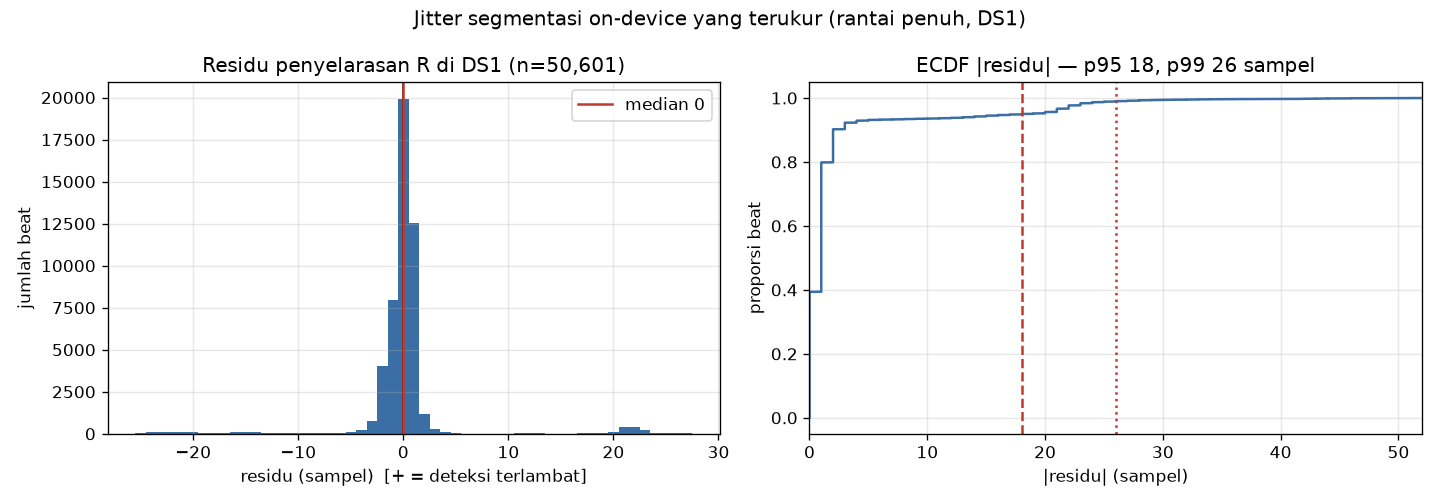
\includegraphics[width=\linewidth,keepaspectratio]{jitter_residu.png}
  \caption{Sebaran residu posisi R-\textit{peak} hasil detektor terhadap anotasi pada DS1}
  \label{fig:residu-jitter}
\end{figure}

Gambar~\ref{fig:residu-jitter} memperlihatkan histogram residu 50.601 pasangan deteksi dan anotasi pada panel kiri serta fungsi distribusi kumulatif empiris (ECDF) nilai mutlaknya pada panel kanan. Intinya tajam di sekitar median 0, yaitu 79,9\% detak meleset paling banyak 1 sampel. Ekornya berat, dengan persentil ke-95 dan ke-99 sebesar 18 dan 26 sampel yang ditandai garis vertikal, serta residu terbesar 54 sampel atau sekitar 150 ms. Ekor ini terkumpul pada rekaman berderau 108, 203, dan 207. Bentuk ini berbeda dari \textit{jitter} seragam $\pm$18 sampel pada Dias et al.~\cite{dias_2021}, karena itu augmentasi mengambil ulang residu terukur.
% sumber: gambar laporan/buku-pa/gambar/jitter_residu.png (dibuka dan dibaca); model/artifacts/metrics/jitter/residu_ds1.npy (50.601 residu, median 0, |r| <= 1 0,7985, |r| <= 2 0,9022, p95 18, p99 26, maks 54); model/artifacts/metrics/jitter/jitter_residu.csv (std 108 14,771, 203 10,792, 207 17,434); 54 / 360 = 0,150 detik; model/docs/jitter-walkthrough.md bagian 2 (paper memakai jitter seragam delta <= 18 sampel)

Pada model lama, yaitu \textit{window} 250 sampel tanpa augmentasi dengan \textit{threshold} 0,35, menggeser posisi R pada DS2 mengikuti sebaran ini menurunkan F1 dari 0,5659 menjadi 0,4534. AUC hanya turun dari 0,8866 menjadi 0,8586, jadi urutan probabilitas nyaris utuh dan yang rusak adalah titik operasinya. Pergeseran seragam 4 sampel saja sudah menurunkan F1 menjadi 0,3170, karena tiga lapisan \textit{max pooling} berukuran 2 membuat pergeseran 4 sampel setara setengah \textit{bin pooling}. Model karena itu dilatih ulang dengan dua salinan DS1 ber-\textit{jitter} empiris, dan pada model hasil latih ulang tersebut F1 dengan segmentasi detektor hanya berselisih 0,0095 dari F1 dengan segmentasi anotasi (Tabel~\ref{tab:segmentasi-deteksi}).

% sumber: rerata lima seed dari model/artifacts/metrics/jitter/sweep_jitter_dasar.csv (n 49.654 = DS2 versi window 250; delta 0: f1 0,5659 auc 0,8866; delta 4 seragam: f1 0,3170; empiris: f1 0,4534 auc 0,8586); model/docs/jitter-walkthrough.md bagian 4 (model Fase 5 threshold 0,35, kerusakan pada titik operasi); model/CLAUDE.md jebakan "Model runtuh kalau R-peak meleset 4 sampel" (stride total 8)

\subsubsection{Ablasi dan Keputusan Rancangan}

Setiap pilihan pengaturan model diputuskan dari pengukuran. Setiap varian melewati rantai yang sama, yaitu menyusun DS1 sesuai varian, melatih, mengalibrasi \textit{threshold} pada VAL, lalu mengukur DS2. Hanya satu pengaturan yang diubah per varian, dengan paling sedikit tiga \textit{seed}, dan hasilnya berupa rerata beserta setengah rentang. Selisih F1 di bawah 0,04 tidak dianggap bermakna, karena penjadwalan \textit{thread} oneDNN membuat hasil berubah walaupun \textit{seed} sama. Rerata tiga \textit{seed} konfigurasi terkunci pun bergeser dari 0,6911 menjadi 0,6535 saat diulang pada pengulangan kedua, dan F1 model akhir \textit{float32} sebesar 0,6594 berada dalam rentang pengulangan kedua, yaitu 0,6261 sampai 0,6821. Keputusan Dipilih diberikan pada varian yang dipakai dan Acuan pada varian pembanding. Keputusan Ditolak diberikan pada varian yang tidak dipakai, baik karena lebih buruk, menukar kelas yang lebih penting, maupun menambah biaya tanpa selisih bermakna. Hasil yang menentukan keputusan dirangkum pada Tabel~\ref{tab:ablasi}.
% sumber: model/docs/jitter-walkthrough.md bagian 5 (rantai ablasi, threshold per varian dari VAL, ukur DS2); model/scripts/ringkas_ablasi.py (SEED_MINIMAL 3, rerata dan setengah-rentang, AMBANG = 0.04); model/docs/arsip/2026-09-18-robustness-changelog.md bagian B2 (0,6209 vs 0,5882); keluaran ringkas_ablasi.py (w128b 0,6911, t8_lr1e3 0,6535); model/artifacts/metrics/ablasi/ablasi.csv (seed 42, 7, 13, ditambah 21, 34, 55 pada sebagian varian; t8_lr1e3 per seed 0,626084, 0,682129, 0,652266); model/artifacts/metrics/fase6_metrics_fp32.csv (f1 0,659403); model/src/dataset.py bagi_train_test (held-out sorted()[::4], sisanya ke latih); model/CLAUDE.md decision "Database LATIH" (mitdb saja)

\begin{table}[!ht]
  \centering
  \caption{Ringkasan ablasi yang menentukan keputusan rancangan, dinilai pada DS2}
  \label{tab:ablasi}
  \setstretch{1.0}
  \setlength{\tabcolsep}{3pt}
  \renewcommand{\arraystretch}{1.15}
  \small
  \begin{tabularx}{\linewidth}{>{\RaggedRight\arraybackslash}p{0.9cm}>{\RaggedRight\arraybackslash}X>{\centering\arraybackslash}p{0.9cm}>{\centering\arraybackslash}p{2.6cm}>{\raggedleft\arraybackslash}p{1.2cm}>{\raggedleft\arraybackslash}p{1.2cm}>{\centering\arraybackslash}p{1.9cm}}
    \toprule
    \textbf{ID} & \textbf{Perubahan terhadap Acuan} & \textbf{\textit{Seed}} & \textbf{F1 DS2} & \textbf{\textit{Recall} S} & \textbf{AUC} & \textbf{Keputusan} \\
    \midrule
    \multicolumn{7}{l}{\textit{Augmentasi jitter, window 90/160}} \\
    A1 & Tanpa augmentasi & 3 & 0,5660 $\pm$0,0202 & 0,2683 & 0,8870 & Acuan \\
    \textbf{A2} & \textbf{\textit{Jitter} $\times$2} & \textbf{3} & \textbf{0,6354 $\pm$0,0428} & \textbf{0,2712} & \textbf{0,9084} & \textbf{Dipilih} \\
    \midrule
    \multicolumn{7}{l}{\textit{Posisi R dalam window, jitter $\times$2}} \\
    A3 & 128/127 & 3 & 0,6775 $\pm$0,0112 & 0,4871 & 0,9394 & Ditolak \\
    A4 & 112/144 & 3 & 0,5786 $\pm$0,0311 & 0,3691 & 0,9069 & Ditolak \\
    \textbf{A6} & \textbf{128/128} & \textbf{3} & \textbf{0,6911 $\pm$0,0290} & \textbf{0,4221} & \textbf{0,9373} & \textbf{Dipilih} \\
    \midrule
    \multicolumn{7}{l}{\textit{Jumlah salinan jitter, window 128/127}} \\
    A7 & \textit{Jitter} $\times$3 & 3 & 0,6099 $\pm$0,0254 & 0,3807 & 0,9146 & Ditolak \\
    \midrule
    \multicolumn{7}{l}{\textit{Fitur HOS, window 90/160, jitter $\times$2}} \\
    A5 & $+$ HOS & 3 & 0,6150 $\pm$0,0509 & 0,3123 & 0,8882 & Ditolak \\
    \midrule
    \multicolumn{7}{l}{\textit{Fitur ritme tambahan pada A6}} \\
    A8 & $+$ rasio R-R, lebar QRS & 4 & 0,6882 $\pm$0,0233 & 0,4203 & 0,9228 & Ditolak \\
    \midrule
    \multicolumn{7}{l}{\textit{Learning rate, pengulangan kedua A6}} \\
    A9 & LR $10^{-3}$ & 3 & 0,6535 $\pm$0,0280 & 0,4473 & 0,9305 & Acuan \\
    A10 & LR $10^{-4}$ & 3 & 0,6729 $\pm$0,0483 & 0,3126 & 0,9415 & Ditolak \\
    \bottomrule
  \end{tabularx}
  \par\vspace{2pt}{\footnotesize\raggedright Keterangan: angka a/b menyatakan jumlah sampel sebelum dan sesudah R, $\times$2 dan $\times$3 adalah jumlah salinan \textit{jitter}, $\pm$ adalah setengah rentang antar-\textit{seed}, HOS adalah kurtosis dan \textit{skewness}, dan LR adalah \textit{learning rate}. Baris tebal adalah varian yang dipakai. A8 Ditolak karena F1-nya tidak berbeda bermakna dari A6 sedangkan \textit{recall} V turun. A10 Ditolak karena \textit{recall} S turun walaupun AUC naik. Hanya varian yang menentukan keputusan dengan paling sedikit tiga \textit{seed} yang ditampilkan.\par}
\end{table}
% ID varian -> tag di model/artifacts/metrics/ablasi/ablasi.csv: A1 bersih, A2 jitter, A3 w128, A4 w112, A5 hos, A6 w128b, A7 w128s3, A8 fd_mitdb_only, A9 t8_lr1e3, A10 t8_lr1e4
% sumber: keluaran model/.venv/bin/python model/scripts/ringkas_ablasi.py (F1 rerata +- setengah-rentang, recall S rerata, AUC rerata, kolom n = jumlah seed); konfigurasi per tag dari model/artifacts/metrics/ablasi/ablasi.csv (win_pre, win_post, hos, jitter, salinan, n_train); arti fb_ dan fd_ dari model/docs/arsip/2026-09-19-faseB-changelog.md bagian 1 dan 9 serta git show ad82617 (PA_RR_RATIO, PA_QRSW); vonis mengikuti model/CLAUDE.md tabel decision point ("Ukuran window", "Augmentasi jitter", "Fitur HOS", "Database LATIH", "Bentuk fitur ritme", "Learning rate"); tag dengan seed < 3 (g_diag, g_diagbase, g_lrdiag) tidak dimasukkan; baris g_lr1e4 (setara t8_lr1e4 pada batch pertama) dan fd_rr (tercakup fd_both) dikeluarkan untuk meringkas; vonis hos Ditolak mengikuti model/CLAUDE.md "Fitur HOS", w128 Ditolak karena window 128/127 tidak dipakai (255 sampel, w128b 128/128 yang terkunci)

Dua keputusan terbesar pada Tabel~\ref{tab:ablasi} adalah augmentasi \textit{jitter} dan \textit{window} 128/128. Augmentasi \textit{jitter} menaikkan F1 dari 0,5660 menjadi 0,6354 walaupun DS2 tidak diberi \textit{jitter}, jadi augmentasi bekerja sebagai regularisasi. \textit{Window} dengan 128 sampel sebelum R menaikkan F1 lebih jauh dan hampir menggandakan \textit{recall} S, sedangkan A4 yang sama-sama berpanjang 256 sampel dengan konteks sebelum R lebih pendek justru turun di bawah A2. Yang memberi manfaat karena itu adalah konteks sebelum R yang memuat gelombang P dan interval PR. Varian 128/128 setara dengan 128/127 dan dipilih karena 256 habis dibagi 8.

Biaya \textit{window} 128/128 terletak pada kelas F, yang \textit{recall}-nya turun dari 0,3084 pada acuan menjadi 0,1521. Sebagian besar penurunan itu sudah terjadi saat augmentasi \textit{jitter} ditambahkan (0,1692), jadi biaya \textit{window} sendiri kecil. Biaya ini diterima karena DS2 memuat 1.836 detak S dan hanya 388 detak F.

Fitur rasio R-R dan lebar QRS (A8) tidak menaikkan F1 secara bermakna, tetapi menurunkan \textit{recall} V dari 0,9437 menjadi 0,8983. A8 karena itu ditolak.

% sumber: tab:ablasi; model/CLAUDE.md decision "Ukuran window" (w112 sebagai isolator, konteks pre-R, gelombang P dan interval PR), "Fitur HOS", "Database LATIH", "Bentuk fitur ritme"; model/docs/arsip/2026-09-18-robustness-changelog.md bagian F1 (w128 255 sampel vs w128b 256, rantai pooling 256-128-64-32) dan F2 (3 salinan lebih buruk); rerata dari model/artifacts/metrics/ablasi/ablasi.csv (anot_recall_F bersih 0,3084, w128b 0,1521; anot_recall_V w128b 0,9437, fd_mitdb_only 0,8983); jumlah S dan F DS2 dari perhitungan ulang per kelas pada butir evaluasi DS2 (1.836 dan 388); model/docs/arsip/2026-09-19-faseB-changelog.md bagian 2 dan 9
% sumber: recall F per varian dari rerata anot_recall_F di model/artifacts/metrics/ablasi/ablasi.csv (bersih 0,308419, jitter 0,169244, w128b 0,152062; penurunan jitter 0,1392 dari total 0,1564 = 89%); varian yang tidak ditampilkan dari keluaran ringkas_ablasi.py (fb_multi 0,6419, fb_svdb_nocw 0,6223, fd_qrsw 0,6503, fd_rr 0,6853, g_swa3 0,6346, g_lr1e4 0,6827, t8_lr3e4 0,6421, semuanya di bawah varian terkunci pada kelompok batch-nya; g_diag, g_diagbase, g_lrdiag hanya 1 seed)

\textit{Learning rate} $10^{-4}$ menghasilkan pertukaran yang disengaja. AUC DS2 naik pada kedua pengulangan dan \textit{recall} F DS2 naik dari 0,1804 menjadi 0,3591, sedangkan F1 DS2 tidak berbeda bermakna. Sebaliknya, \textit{recall} S DS2 turun dari 0,4473 menjadi 0,3126. Penurunan ini bukan efek \textit{threshold}, karena pada \textit{recall} total yang disamakan, $10^{-3}$ tetap unggul pada kelas S di keenam perbandingan pada \textit{seed} 42, sedangkan penyebab pastinya belum diketahui.

\textit{Learning rate} $10^{-3}$ dipertahankan karena dua alasan. Pertama, kelas S paling bergantung pada ritme dan konteks sebelum R, dan kelas ini menjadi alasan rancangan \textit{hybrid}. Kedua, perpindahan menuntut pembuatan ulang berkas model pada \textit{firmware} beserta validasi ulang di perangkat. Model hasil satu \textit{epoch} karena itu tercatat sebagai keterbatasan yang disengaja.
% sumber: tab:ablasi (t8_lr1e3 AUC 0,9305 dan F1 0,6535, t8_lr1e4 AUC 0,9415 dan F1 0,6729, recall S t8 0,4473 dan 0,3126); keluaran ringkas_ablasi.py (w128b AUC 0,9373 dan g_lr1e4 AUC 0,9461 sebagai batch pertama, baris keduanya dikeluarkan dari tab:ablasi); selisih F1 DS2 0,6729 - 0,6535 = 0,0194 di bawah ambang 0,04; rerata anot_recall_F di model/artifacts/metrics/ablasi/ablasi.csv (t8_lr1e3 0,1804, t8_lr1e4 0,3591); model/docs/arsip/2026-09-19-faseG-changelog.md bagian 4 (threshold tetap dari VAL, uji titik operasi setara model/scripts/cek_titik_operasi.py pada DS2 test.npz hanya seed 42 pada recall total 0,65/0,70/0,80, 6 dari 6) dan bagian 8; model/CLAUDE.md decision "Learning rate" (TETAP 1e-3, biaya regen model_int8.h dan golden_ref.h serta validasi board saat HW-5 buntu)

\subsubsection{Kuantisasi INT8}

Model INT8 yang dievaluasi pada DS2 adalah hasil kuantisasi varian \textit{deploy}, yaitu DepthwiseConv1D(32) berbobot 1/32 sebagai pengganti \textit{Global Average Pooling} dengan kepala Conv1D \textit{kernel} 1. Kuantisasinya memakai \textit{post-training quantization} INT8 penuh dengan 300 sampel kalibrasi \textit{stratified} dari DS1.
% sumber: model/src/model.py build_deploy_model (kernel = panjang sesudah tiga pooling = 32, bobot 1/32, Conv1D kernel 1); model/artifacts/model_int8.tflite (tensor gap_dw [1,1,32,32]); model/config.py (REP_SAMPLES 300, INT8_IO True); model/src/quantize.py (stratified, inference_input_type dan output_type int8)

Kuantisasi memenuhi target, karena F1 model INT8 sebesar 0,6604 mencapai 100,14\% F1 model \textit{float32} sebesar 0,6594, di atas syarat 99\%. Satu-satunya metrik di bawah 99\% adalah \textit{precision}, yaitu 98,93\% nilai \textit{float32}. Penurunan itu sejalan dengan kenaikan \textit{recall}, karena probabilitas yang bergeser di sekitar \textit{threshold} menangkap lebih banyak aritmia sekaligus menambah alarm palsu.
% sumber: model/artifacts/metrics/fase7_delta.csv (f1 0,659403 / 0,660356; precision 0,623549 / 0,616855; recall 0,699633 / 0,710459); rasio int8 / float32 x 100 (f1 100,14; precision 98,93; recall 101,55; specificity 99,75; mcc 100,18; auc 100,10; accuracy 99,90); keputusan user 1 Nov 2026: tabel selisih diringkas ke kalimat

Selisih per kelas searah dengan selisih agregat, dan tidak ada kelas yang turun. \textit{Recall} kelas S, V, dan F masing-masing naik 0,0240, 0,0034, dan 0,0103. Label akhir hanya berubah pada 272 detak, yaitu 0,55\% DS2. Kedua \textit{confusion matrix} dibandingkan pada Gambar~\ref{fig:cm-ds2}.
% sumber: model/artifacts/metrics/fase7_metrik_tambahan.csv (recall_S 0,438998 / 0,462963 / +0,023965; recall_V 0,924821 / 0,928239 / +0,003417; recall_F 0,067010 / 0,077320 / +0,010309; label_berubah 272 dari 49.656 = 0,55%), model/scripts/metrik_tambahan.py; model/docs/quantize-walkthrough.md bagian 6

\begin{figure}[H]
  \centering
  \begin{minipage}{0.4\linewidth}
    \centering
    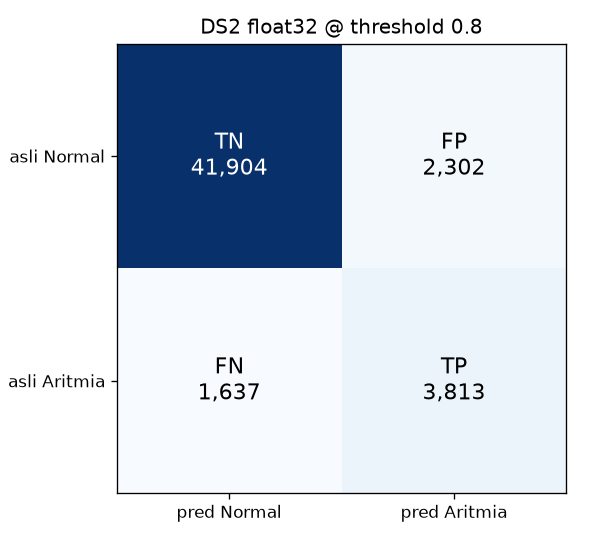
\includegraphics[width=\linewidth,keepaspectratio]{fase6_confusion_fp32.png}\\
    \small (a)
  \end{minipage}\hspace{0.05\linewidth}
  \begin{minipage}{0.4\linewidth}
    \centering
    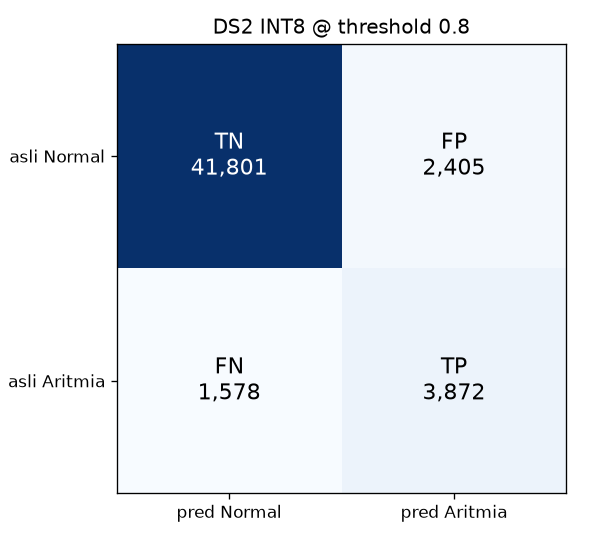
\includegraphics[width=\linewidth,keepaspectratio]{fase7_confusion_int8.png}\\
    \small (b)
  \end{minipage}
  \caption{\textit{Confusion matrix} DS2 pada \textit{threshold} 0,80, (a) model \textit{float32} dan (b) model INT8}
  \label{fig:cm-ds2}
\end{figure}

Pada Gambar~\ref{fig:cm-ds2}, baris adalah label sebenarnya dan kolom adalah prediksi. Model INT8 pada panel (b) menemukan 3.872 detak Aritmia, 59 lebih banyak daripada model \textit{float32} pada panel (a), dengan tambahan 103 FP dari 2.302 menjadi 2.405. Hasil kuantisasi ini bergantung pada varian \textit{deploy} yang dipakai. AveragePooling1D sempat dicoba sebagai pengganti, tetapi menurunkan \textit{recall} DS2 model versi lama dari 0,655 menjadi 0,528 karena operasi \textit{pooling} mewarisi skala kuantisasi masukannya.
% sumber: gambar laporan/buku-pa/gambar/fase6_confusion_fp32.png (TN 41.904, FP 2.302, FN 1.637, TP 3.813) dan fase7_confusion_int8.png (TN 41.801, FP 2.405, FN 1.578, TP 3.872), keduanya dibuka dan dibaca; 3.872 - 3.813 = 59; 2.405 - 2.302 = 103
% sumber: model/CLAUDE.md jebakan "Op pooling mewarisi skala kuantisasi input" (recall DS2 0,655 -> 0,528, skala input diwarisi)

\subsubsection{Kinerja di Perangkat}

Model INT8 harus memenuhi batas waktu dan memori di ESP32-S3. Seluruh kasus uji di \textit{board} lulus, yaitu 16 kasus pada 18 September 2026 dan 29 kasus pada 13 Oktober 2026 setelah uji perangkat dan uji integrasi ditambahkan. Latensi diukur pada 18 September 2026 atas tujuh detak acuan pada CPU 240 MHz dengan \textit{kernel} referensi TensorFlow Lite Micro tanpa ESP-NN. RAM dan Flash diambil dari laporan \textit{build} PlatformIO. Hasilnya ditunjukkan pada Tabel~\ref{tab:sumber-daya}.
% sumber: firmware/test/test_inference/test_inference.cpp test_latensi_dan_memori (rata-rata us_terpakai atas GOLDEN_RR_FIRST sampai GOLDEN_N_BEAT = 7 detak, arena_used_bytes, ESP.getFreeHeap, getCpuFreqMHz); model/docs/firmware-walkthrough.md bagian 6 (240 MHz, kernel referensi tanpa ESP-NN); model/CLAUDE.md HW-1 dan HW-6 (pio test -e esp32-s3 16/16, angka diperbarui 18 Sep 2026); git log f6042b5 dan 07a5a07 (13 Okt 2026, board 29/29; angka latensi tidak dicatat ulang)

\begin{table}[!ht]
  \centering
  \caption{Pemakaian sumber daya model INT8 dan \textit{firmware} di ESP32-S3}
  \label{tab:sumber-daya}
  \setstretch{1.0}
  \setlength{\tabcolsep}{4pt}
  \renewcommand{\arraystretch}{1.15}
  \small
  \begin{tabularx}{\linewidth}{>{\RaggedRight\arraybackslash}X>{\raggedleft\arraybackslash}p{1.8cm}>{\RaggedRight\arraybackslash}X>{\RaggedRight\arraybackslash}p{2.6cm}}
    \toprule
    \textbf{Besaran} & \textbf{Nilai} & \textbf{Kondisi Pengukuran} & \textbf{Target} \\
    \midrule
    Ukuran model INT8 (byte) & 23.488 & Format TensorFlow Lite, \textit{window} 256 & Muat di \textit{flash} \\
    Latensi inferensi per detak (ms) & 26,6 & Uji perangkat, 240 MHz, \textit{kernel} referensi, \textit{window} 256 & Lebih kecil dari interval antardetak \\
    \textit{Tensor arena} terpakai (byte) & 12.948 & Uji perangkat, alokasi 24.576 byte & Muat di SRAM \\
    \textit{Heap} bebas (byte) & 312.396 & Uji perangkat, \textit{window} 256 & Muat di SRAM \\
    RAM statis tanpa MQTT (byte) & 74.284 & \textit{Firmware} tanpa MQTT, dengan tabel \textit{replay} & Muat di memori \\
    Flash tanpa MQTT (byte) & 430.569 & \textit{Firmware} tanpa MQTT, dengan tabel \textit{replay} & Muat di memori \\
    RAM statis dengan MQTT (byte) & 121.336 & \textit{Firmware} dengan MQTT, kredensial WiFi terisi & Muat di memori \\
    Flash dengan MQTT (byte) & 887.873 & \textit{Firmware} dengan MQTT, kredensial WiFi terisi & Muat di memori \\
    \bottomrule
  \end{tabularx}
  \par\vspace{2pt}{\footnotesize\raggedright Keterangan: 23.488 byte setara 22,94 KB atau 0,36\% partisi aplikasi 6,25 MB, dan alokasi \textit{tensor arena} 24.576 byte setara 7,5\% RAM 320 KB. RAM statis 74.284 dan 121.336 byte setara 22,7\% dan 37,0\% dari RAM 320 KB, sedangkan Flash 430.569 dan 887.873 byte setara 6,6\% dan 13,5\% dari partisi aplikasi 6,25 MB.\par}
\end{table}
% sumber: 23.488 / (6,25 x 1.048.576) = 0,358%; 24.576 / (320 x 1.024) = 7,5%; flash 16 MB dari datasheet ESP32-S3-WROOM-1 (N16R8), SRAM 512 KB dari datasheet ESP32-S3; standar batas ukuran model tidak ditemukan (docs/2026-11-01-crosscheck-metrik-bab4/tinyml.md butir 4: MLPerf Tiny tidak menjadikan memori skor)
% sumber: model/docs/firmware-walkthrough.md bagian 6 (inferensi 26,6 ms, tensor arena 12.948 dari 24.576, model 22,94 KB, heap bebas 312.396, RAM 74.284 byte 22,7% dari 320 KB, Flash 430.569 byte 6,6% dari 6,25 MB); model/CLAUDE.md HW-1 (26,6 ms, 12.948 B, 312.396 B); model/docs/firmware-walkthrough.md bagian 6 dan model/docs/mqtt-walkthrough.md bagian 7 (build firmware utama dengan MQTT dan kredensial terisi: RAM 37,0% 121.336 B, Flash 13,5% 887.873 B; angka tanpa kredensial tidak dipakai; nilai lama 36,9% 121.008 B dan 881.861 B diperbarui 13 Okt 2026); firmware/src/klasifikasi.cpp ARENA_N = 24 * 1024; laporan/buku-pa/bab/bab3.tex tab:pengujian-model (target)

Seluruh besaran pada Tabel~\ref{tab:sumber-daya} memenuhi target, jadi model INT8 layak dijalankan secara \textit{on-device} tanpa \textit{cloud}. Latensi 26,6 ms setara paling banyak 13,3\% dari periode refraktori detektor 200 ms, yaitu interval antardetak terpendek, dan sekitar 4,4\% waktu CPU untuk inferensi saja pada laju \textit{replay} sekitar 1,6 detak per detik. \textit{Tensor arena} terpakai 52,7\% dari alokasinya.

RAM statis naik dari 22,7\% menjadi 37,0\% dan Flash dari 6,6\% menjadi 13,5\% karena tumpukan WiFi dan klien MQTT ikut di-\textit{link}. Angka ini hanya sah bila kredensial WiFi terisi. Keterbatasannya, latensi diukur tanpa WiFi aktif.
% sumber: tab:sumber-daya; firmware/include/ecg_preproc.h ECG_PT_REFRACTORY 72 sampel = 200 ms pada 360 Hz dan model/config.py PT_REFRACTORY_MS 200; 26,6 / 200 = 0,133; model/CLAUDE.md status HW-7 Replay dan model/docs/firmware-walkthrough.md §5c (11 detak per putaran 6,67 detik = 1,65 detak per detik), 26,6 x 11 / 6.670 = 0,044; 12.948 / 24.576 = 0,527; model/docs/firmware-walkthrough.md bagian 6 (320 KB, 6,25 MB)

\section{Analisis Hasil Eksperimen}

Hasil eksperimen pada laporan tahap ini dinilai terhadap dua tujuan penelitian, yaitu jalur preprocessing \textit{real-time} dan jalur model TinyML \textit{on-device}. Status Tercapai diberikan bila seluruh target pada rencana pengujian terukur dan terpenuhi, sedangkan Sebagian tercapai diberikan bila ada target yang belum terukur. Kedua jalur berstatus Tercapai. Penilaian per target dirangkum pada Tabel~\ref{tab:ketercapaian}.
% sumber: tab:kualitas-rekaman (4 dari 4 rekaman resmi Berhasil) melengkapi target jalur preprocessing

\begin{table}[!ht]
  \centering
  \caption{Ketercapaian tujuan penelitian}
  \label{tab:ketercapaian}
  \setstretch{1.0}
  \setlength{\tabcolsep}{3pt}
  \renewcommand{\arraystretch}{1.15}
  \small
  \begin{tabularx}{\linewidth}{>{\RaggedRight\arraybackslash}p{2.6cm}>{\RaggedRight\arraybackslash}X>{\RaggedRight\arraybackslash}X>{\centering\arraybackslash}p{2.1cm}}
    \toprule
    \textbf{Tujuan} & \textbf{Target} & \textbf{Hasil} & \textbf{Status} \\
    \midrule
    \multirow{2}{=}{Preprocessing \textit{real-time}} & Tanpa sampel hilang & Sampel hilang 0, beban 3,0\% anggaran & \multirow{2}{=}{\centering Tercapai} \\
    & Sinyal tubuh lolos indeks kualitas sinyal & 92 dari 92 jendela 10 detik, satu sesi & \\
    % sumber: bab4 tab:beban-komputasi, tab:kualitas-rekaman; target dari bab3 tab:pengujian-model dan bab4 tab:parameter-eksperimen baris d dan e
    \midrule
    \multirow{3}{=}{Model INT8 \textit{on-device}} & F1 INT8 minimal 99\% F1 \textit{float32} & 100,14\% & \multirow{3}{=}{\centering Tercapai} \\
    & Latensi di bawah interval antardetak & 26,6~ms per detak & \\
    & Muat di memori ESP32-S3 & Model 0,36\% partisi aplikasi, \textit{arena} 12.948 dari 24.576 byte & \\
    % sumber: bab4 tab:delta-int8, tab:sumber-daya; target dari bab3 tab:pengujian-model
    \bottomrule
  \end{tabularx}
  \par\vspace{2pt}{\footnotesize\raggedright Keterangan: satuan Hasil mengikuti satuan Target pada baris yang sama. F1 INT8 0,6604 terhadap F1 \textit{float32} 0,6594. Jalur \textit{pipeline edge-to-cloud} belum dinilai pada laporan tahap ini.\par}
\end{table}

Seluruh target jalur preprocessing dan jalur model, yaitu target komputasi, model, dan kualitas sinyal tubuh, terpenuhi (Tabel~\ref{tab:ketercapaian}). Target pengiriman data pada rencana pengujian \textit{pipeline}, yaitu PDSR, latensi, bufer lokal, waktu \textit{flush}, dan deduplikasi, belum dinilai karena hasil pengujiannya belum termasuk dalam laporan tahap ini.

\subsection{Analisis Jalur Preprocessing \textit{Real-Time}}

Jalur komputasi preprocessing berjalan secara \textit{real-time} di ESP32-S3. Beban rata-rata hanya 82 $\mu$s per sampel atau 3,0\% anggaran, dan sampel hilang tetap 0 walaupun puncak beban sesaat mencapai 33,4~ms (Tabel~\ref{tab:beban-komputasi}). ADC yang dibaca di ISR dan antrean 256 sampel menyerap \textit{burst} deteksi dan inferensi, dan syarat pada Tabel~\ref{tab:pengujian-model} terpenuhi.
% sumber: bab4 tab:beban-komputasi (82 us, 3,0%, 33,4 ms, sampel hilang 0, antrean 256), sec:karakteristik-data butir penyelarasan (berkas ecg_preproc.h dan model_int8.h dihasilkan otomatis)

Sinyal tubuh juga layak sebagai masukan jalur ini, karena keempat rekaman resmi dari satu sesi perekaman lolos indeks kualitas sinyal pada seluruh jendela (Tabel~\ref{tab:kualitas-rekaman}). Segmentasi hasil detektor tidak merusak klasifikasi, dengan F1 0,6499 dibandingkan 0,6594 pada segmentasi anotasi (Tabel~\ref{tab:segmentasi-deteksi}). Catatannya, beban rata-rata diukur pada sinyal \textit{replay} sepanjang 6,67 detik dengan model \textit{window} 250, dan detektor menemukan kelas S dengan \textit{sensitivity} 0,6494 (Tabel~\ref{tab:sensitivity-detektor}). Sinyal tubuh juga baru berasal dari satu subjek dan satu sesi. Karena seluruh target jalur ini terpenuhi pada pengujian yang dilakukan, jalur preprocessing dinilai Tercapai dengan cakupan tersebut dicatat sebagai keterbatasan.
% sumber: bab4 subsec:hasil-tujuan1 butir port C (rekaman 208, 6,67 detik, tanpa kelas S) dan butir alur hidup (window 250), tab:sensitivity-detektor (S 0,6494), tab:segmentasi-deteksi

\subsection{Analisis Jalur Model TinyML \textit{On-Device}}

Model INT8 berjalan secara \textit{on-device} di ESP32-S3 dalam batas waktu dan memori yang ditargetkan. Kuantisasi mempertahankan F1 pada 100,14\% nilai \textit{float32} dengan ukuran model 22,94~KB. Inferensi memakan 26,6~ms per detak atau paling banyak 13,3\% dari interval antardetak terpendek 200~ms, dan \textit{tensor arena} terpakai 12.948 dari 24.576 byte (Tabel~\ref{tab:sumber-daya}). Hasil ini bergantung pada varian \textit{deploy} berbasis DepthwiseConv1D, karena operasi MEAN pada TensorFlow Lite Micro salah hitung tanpa pesan kesalahan.
% sumber: bab4 tab:delta-int8 (+0,0108, 22,94 KB), tab:sumber-daya dan paragraf sesudahnya (26,6 ms, 13,3% dari 200 ms, 12.948 dari 24.576 byte), subsec:hasil-tujuan1 336 vs 0,973)

Kualitas klasifikasi, yang tidak memiliki ambang angka, mencapai \textit{recall} 0,7105, F1 0,6604, dan AUC 0,9344 pada model INT8 (Tabel~\ref{tab:hasil-ds2}) dengan median \textit{recall} per pasien 0,9167. Kelemahan terbesarnya adalah kelas S dengan \textit{recall} 0,4630, karena QRS-nya mirip Normal dan pembedanya terletak pada waktu kedatangan serta gelombang P. Latensi inferensi diukur tanpa WiFi aktif. Jalur model dinilai Tercapai, karena target kuantisasi, ukuran, latensi, dan memori seluruhnya terpenuhi.
% sumber: bab4 tab:hasil-ds2 (0,6996, 0,6594, 0,9334), subsec:hasil-tujuan2 butir Evaluasi DS2 (median per pasien 0,9167, recall S 0,4390, alasan QRS mirip Normal), butir Konsumsi Daya (INA219 belum dirakit di sisi baterai), paragraf sesudah tab:sumber-daya (latensi tanpa WiFi aktif)

\subsection{Perbandingan dengan Penelitian Terkait}

Perbandingan dibatasi pada penelitian terkait yang skema evaluasinya diketahui, yaitu Zambrano-de la Torre et al.~\cite{zambrano_2026} dan penelitian pendahulu~\cite{mulyawan_2026} yang memakai platform sensor dan \textit{dashboard} yang sama. Protokol ketiganya disandingkan pada Tabel~\ref{tab:perbandingan-protokol}.

\begin{table}[!ht]
  \centering
  \caption{Perbandingan protokol evaluasi dengan penelitian terkait}
  \label{tab:perbandingan-protokol}
  \setstretch{1.0}
  \setlength{\tabcolsep}{3pt}
  \renewcommand{\arraystretch}{1.15}
  \small
  \begin{tabular}{>{\RaggedRight\arraybackslash}p{2.3cm}>{\RaggedRight\arraybackslash}p{2.0cm}>{\RaggedRight\arraybackslash}p{2.5cm}>{\RaggedRight\arraybackslash}p{2.4cm}>{\RaggedRight\arraybackslash}p{3.5cm}}
    \toprule
    \textbf{Penelitian} & \textbf{Kelas} & \textbf{Pembagian Data} & \textbf{Lokasi Inferensi} & \textbf{Hasil yang Dilaporkan} \\
    \midrule
    Zambrano-de la Torre et al.~\cite{zambrano_2026} &
    Tiga kelas, yaitu N, V, dan S &
    Per detak tanpa pemisahan antarpasien pada MIT-BIH &
    Arduino UNO 8-bit, 1D-CNN INT8 &
    \textit{Accuracy}, degradasi kuantisasi $<$ 0,7\%, model $<$ 22~KB, latensi sekitar 200~ms per detak \\
    % sumber: bab2 subsec:related-zambrano2026 dan tab:perbandingan-penelitian baris 11
    Penelitian pendahulu~\cite{mulyawan_2026} &
    Atrial fibrilasi &
    Pengujian \textit{offline}, dilatih pada MIT-BIH &
    SVM di \textit{backend cloud}, ESP32 untuk akuisisi dan fitur R-R &
    \textit{Accuracy} tinggi pada pengujian \textit{offline} \\
    % sumber: bab2 subsec:related-mulyawan2026 dan tab:perbandingan-penelitian baris 12 (tanpa angka akurasi)
    Penelitian ini &
    Biner, yaitu Normal dan Aritmia &
    \textit{Inter-patient} DS1/DS2, DS2 berisi 22 pasien &
    ESP32-S3, model \textit{hybrid} INT8 \textit{on-device} &
    INT8 pada DS2 \textit{recall} 0,7105, F1 0,6604, AUC 0,9344, \textit{accuracy} 0,9198, model 22,94~KB, latensi 26,6~ms per detak \\
    % sumber: bab4 tab:delta-int8 (INT8), tab:sumber-daya (26,6 ms), subsec:hasil-tujuan2 butir Evaluasi DS2 (22 pasien)
    \bottomrule
  \end{tabular}
\end{table}

Angka ketiga penelitian pada Tabel~\ref{tab:perbandingan-protokol} tidak dapat dibandingkan langsung karena kelas, pembagian data, dan metriknya berbeda. Pembagian per detak membuat detak dari pasien yang sama dapat muncul di himpunan latih dan uji, sedangkan DS2 berisi 22 pasien yang tidak pernah dilihat saat pelatihan. Latensi juga tidak dibandingkan karena Arduino UNO 8-bit dan ESP32-S3 berbeda kelas. Pada sisi metrik, 89,0\% detak DS2 berlabel Normal, jadi menebak Normal untuk seluruh detak sudah memberi \textit{accuracy} sekitar 0,89. \textit{Accuracy} model INT8, yaitu 0,9198, hanya sekitar 3 poin di atasnya (Tabel~\ref{tab:hasil-ds2}). \textit{Accuracy} pada data setimpang ini belum menunjukkan kemampuan mendeteksi aritmia, karena itu hasil penelitian ini dilaporkan melalui \textit{recall}, F1, dan AUC.
% sumber: bab4 sec:parameter-eksperimen (89,0%, sekitar 0,89), subsec:hasil-tujuan2 butir Evaluasi DS2 (accuracy 0,9207 sekitar 3 poin di atas tebak Normal), tab:delta-int8 (0,9207 dan 0,9198)

Penelitian pendahulu mendeteksi atrial fibrilasi dengan SVM di sisi \textit{cloud}~\cite{mulyawan_2026}. Penelitian ini melanjutkannya dengan memindahkan klasifikasi per detak ke ESP32-S3. Protokol \textit{inter-patient} disadari membuat angka penelitian ini tampak lebih rendah daripada \textit{accuracy} pada pembagian per detak~\cite{xiao_2023}, dan angka DS2 pun berpotensi sedikit optimistis karena DS2 dipakai menilai ablasi \textit{window} dan \textit{jitter}. Penelitian ini karena itu tidak mengklaim \textit{accuracy} yang lebih tinggi. Yang diklaim adalah evaluasi yang lebih ketat terhadap pasien baru dan inferensi yang berjalan langsung di perangkat.
% sumber: bab2 subsec:related-mulyawan2026 (SVM di backend cloud, AFib); bab4 tab:sumber-daya (26,6 ms), subsec:hasil-tujuan2 butir Evaluasi DS2 (DS2 menilai ablasi window dan jitter, berpotensi sedikit optimistis), tab:uji-kesetaraan-tahap

\subsection{Keterbatasan dan Status \textit{Proof of Concept}}

Walaupun jalur komputasi dan model INT8 telah terukur di perangkat, sistem ini berstatus \textit{proof of concept} di lingkungan non-klinis dan bukan alat diagnosis, dengan keterbatasan yang diuraikan pada butir berikut.
\begin{enumerate}
  \item Rekaman perangkat berasal dari satu subjek sehat, yaitu penulis, dan variasi sinyal antarindividu belum terwakili.
  \item Rekaman sinyal tubuh resmi berasal dari satu sesi dengan empat rekaman yang seluruhnya memenuhi kriteria (Tabel~\ref{tab:kualitas-rekaman}), dan variasi antarsesi belum terwakili.
  \item Model hanya biner dan tidak menamai jenis aritmia.
  \item \textit{Recall} kelas S masih rendah. \textit{Learning rate} $10^{-3}$ tetap dipakai demi kelas S karena $10^{-4}$ menurunkan \textit{recall} S DS2 dari 0,4473 menjadi 0,3126 walaupun AUC naik (Tabel~\ref{tab:ablasi}), dengan konsekuensi model akhir hasil satu \textit{epoch}.
  \item Angka DS2 berpotensi sedikit optimistis karena DS2 ikut menilai ablasi \textit{window} dan \textit{jitter}.
  \item Gerbang kualitas dengan sinyal tubuh diuji pada satu subjek, dan transisi fase pada kontak baik diamati pada perangkat tanpa log serial.
  \item Deteksi R-\textit{peak} pada sinyal tubuh belum divalidasi terhadap perangkat ECG acuan, jadi hasil akuisisi berupa status fungsional dan bukan akurasi.
\end{enumerate}
% sumber: bab4 sec:karakteristik-data butir data primer, tab:kualitas-rekaman, tab:ablasi (0,4473 dan 0,3126) dan butir Ablasi (satu epoch), butir Evaluasi DS2 (DS2 ikut menilai ablasi window dan jitter, berpotensi sedikit optimistis), subsec:hasil-tujuan1 butir Gerbang Kalibrasi dan butir Segmentasi (0,6661 menjadi 0,5656, window 250)

Sebagian besar keterbatasan tersebut berkaitan dengan cakupan uji, bukan dengan jalur komputasi, dan arah pengembangannya dirangkum sebagai saran pengembangan.
